%
% $RCSfile: cybernetics_oriented_language.tex,v $
%
% Copyright (C) 2002-2008. Christian Heller.
%
% Permission is granted to copy, distribute and/or modify this document
% under the terms of the GNU Free Documentation License, Version 1.1 or
% any later version published by the Free Software Foundation; with no
% Invariant Sections, with no Front-Cover Texts and with no Back-Cover
% Texts. A copy of the license is included in the section entitled
% "GNU Free Documentation License".
%
% http://www.cybop.net
% - Cybernetics Oriented Programming -
%
% http://www.resmedicinae.org
% - Information in Medicine -
%
% Version: $Revision: 1.1 $ $Date: 2008-08-19 20:41:06 $ $Author: christian $
% Authors: Christian Heller <christian.heller@tuxtax.de>
%

\chapter{Cybernetics Oriented Language}
\label{cybernetics_oriented_language_heading}
\index{Cybernetics Oriented Language}
\index{CYBOL}

\begin{flushright}
    \textsl{The Whole is more than the Sum of its Parts.}\\
    \textsc{Aristotle}
\end{flushright}

Chapter \ref{knowledge_schema_heading} introduced a new model for structuring
knowledge, which chapter \ref{state_and_logic_heading} separated into state-
and logic knowledge. What still has to be given though, is a
\emph{Proof of Operability} for these concepts. The following sections will
therefore define the \emph{Cybernetics Oriented Language} (CYBOL), which
contains all new principles and ideas, as first mentioned in \cite{heller2004}.

%
% $RCSfile: formality.tex,v $
%
% Copyright (C) 2002-2008. Christian Heller.
%
% Permission is granted to copy, distribute and/or modify this document
% under the terms of the GNU Free Documentation License, Version 1.1 or
% any later version published by the Free Software Foundation; with no
% Invariant Sections, with no Front-Cover Texts and with no Back-Cover
% Texts. A copy of the license is included in the section entitled
% "GNU Free Documentation License".
%
% http://www.cybop.net
% - Cybernetics Oriented Programming -
%
% http://www.resmedicinae.org
% - Information in Medicine -
%
% Version: $Revision: 1.1 $ $Date: 2008-08-19 20:41:06 $ $Author: christian $
% Authors: Christian Heller <christian.heller@tuxtax.de>
%

\section{Formality}
\label{formality_heading}
\index{Formality}
\index{Informal Language}
\index{Semi-Formal Diagrams}
\index{Formal Programming Language}
\index{Machine Language}
\index{Knowledge Modelling Language}

Abstract models can be described in different ways, for example \cite{philippow}:

\begin{itemize}
    \item[-] \emph{informally} by natural language
    \item[-] \emph{semi-formally} by diagrams
    \item[-] \emph{formally} by a programming language
\end{itemize}

The use of a programming language eases model abstraction for human programmers.
Special tools exist that break down models given in form of programming language
code into their binary form, into sequences of \emph{0} and \emph{1}. These
sequences are called \emph{Machine Language} because they are understood by
computers.

Classical programming languages have the linguistic means to express high-level
\emph{Knowledge} as well as low-level \emph{System Control} operations, such as
those for \emph{input/ output} (i/o), necessary for communication. The use of
such languages inevitably leads to a mess in program code because knowledge and
system control are mixed up. Inflexible, overly complex systems with numerous
interdependencies are the result. Part \ref{basics_heading} of this work
criticised some of the weak points of traditional programming language concepts.

This work makes the necessary split: Knowledge gets \emph{separated} from
system control. Chapter \ref{statics_and_dynamics_heading} already discussed
this separation giving manifold examples, taken from several sciences. The CYBOL
language being described in the next sections is just another form of storing
knowledge. It can therefore also be called a \emph{Knowledge Modelling Language}.
Any other low-level system control functionality belongs to the
\emph{Cybernetics Oriented Interpreter} (CYBOI), which gets introduced in the
later chapter \ref{cybernetics_oriented_interpreter_heading}.

%
% $RCSfile: definition.tex,v $
%
% Copyright (c) 2004. Christian Heller. All rights reserved.
%
% No copying, altering, distribution or any other actions concerning this
% document, except after explicit permission by the author!
% At some later point in time, this document is planned to be put under
% the GNU FDL license. For now, _everything_ is _restricted_ by the author.
%
% http://www.cybop.net
% - Cybernetics Oriented Programming -
%
% http://www.resmedicinae.org
% - Information in Medicine -
%
% @author Christian Heller <christian.heller@tuxtax.de>
%

\subsection{Definition}
\label{definition_heading}

\emph{Patterns}, in a more correct form called \emph{Software Patterns}, represent
solutions for recurring software design problems and can be understood as
recommendations for how to build software in an elegant way. In the past, more
detailed definitions have been given by meanwhile well-known authors.

Christopher Alexander, an architect and urban planner, writes \cite{alexander}:
\textit{Each pattern describes a problem which occurs over and over again in
our environment, and then describes the core of the solution to that problem,
in such a way that you can use this solution a million times over, without ever
doing it the same way twice.} He gave this definition primarily for problems
occuring in architecture, construction, and urban/regional planning, but it can
be applied in the same manner to software design, as done first by Ward
Cunningham and others \cite{portland}.

The systems designer Swift \cite{designmatrix} sees a pattern as:
\textit{essentially a morphological law, a relationship among parts (pattern
components) within a particular context. Specifically, a pattern expresses a
relationship among parts that resolves problems that would exist if the
relationship were missing. As patterns express these relationships, they are
not formulae or algorithms, but rather loose rules of thumb or heuristics.}

The \emph{Gang of Four} (Erich Gamma et al.) applied Alexander's definition to
object oriented software and created a whole catalogue of design patterns
\cite{gamma1995}. After them, patterns are: \textit{Structured models of
thinking that represent reusable solutions for one-and-the-same design problem.
They shall support the development, maintenance and extension of large software
systems, while being independent from concrete implementation languages.} The
experts identified four basic elements of each pattern: \emph{Name},
\emph{Problem}, \emph{Solution} and \emph{Consequences} (advantages and
disadvantages).

For Frank Buschmann et al., software patterns contain the knowledge of
experienced software engineers and help to improve the quality of decision
making \cite{buschmann}. In his opinion, they are \emph{Problem Solution Pairs},
that is basic solutions for problems that already occured in a similar way before.

Martin Fowler means that: \textit{A pattern is some idea that already was
helpful in a practical context and will probably be useful in other contexts,
too.} \cite{fowler1997}. After him, patterns, however they are written, have
four essential parts: \emph{Context}, \emph{Problem}, \emph{Forces} and
\emph{Solution}.

Depending on their experience, software developers produce good or bad solutions.
One possibility to improve less well-done designs or to extend legacy systems
are \emph{Anti-Patterns} (telling how to go from a problem to a bad design),
or the contrasting \emph{Amelioration Patterns} (telling how to go from a bad-
to a good solution) \cite{portland}. Both help finding patterns in wrong-designed
systems, to improve these.

There are efforts to combine patterns to form a \emph{Pattern Language}, also
called \emph{Pattern System} \cite{buschmann}. Such systems describe
dependencies between patterns, specify rules for pattern combination and show
how patterns can be implemented and used in software development practice.

%
% $RCSfile: constructs.tex,v $
%
% Copyright (C) 2002-2008. Christian Heller.
%
% Permission is granted to copy, distribute and/or modify this document
% under the terms of the GNU Free Documentation License, Version 1.1 or
% any later version published by the Free Software Foundation; with no
% Invariant Sections, with no Front-Cover Texts and with no Back-Cover
% Texts. A copy of the license is included in the section entitled
% "GNU Free Documentation License".
%
% http://www.cybop.net
% - Cybernetics Oriented Programming -
%
% http://www.resmedicinae.org
% - Information in Medicine -
%
% Version: $Revision: 1.1 $ $Date: 2008-08-19 20:41:06 $ $Author: christian $
% Authors: Christian Heller <christian.heller@tuxtax.de>
%

\section{Constructs}
\label{constructs_heading}
\index{CYBOL Constructs}

After having defined the CYBOL language in the previous section, the following
examples can demonstrate how the language's constructs may be used in practice.
Attention is also payed to how control structures of classical programming
languages (compare section \ref{structured_and_procedural_programming_heading})
may be implemented in CYBOL. Additionally, this section discusses how
inheritance, containers and software patterns were considered in the design of
CYBOL.

%
% $RCSfile: state_examples.tex,v $
%
% Copyright (C) 2002-2008. Christian Heller.
%
% Permission is granted to copy, distribute and/or modify this document
% under the terms of the GNU Free Documentation License, Version 1.1 or
% any later version published by the Free Software Foundation; with no
% Invariant Sections, with no Front-Cover Texts and with no Back-Cover
% Texts. A copy of the license is included in the section entitled
% "GNU Free Documentation License".
%
% http://www.cybop.net
% - Cybernetics Oriented Programming -
%
% http://www.resmedicinae.org
% - Information in Medicine -
%
% Version: $Revision: 1.1 $ $Date: 2008-08-19 20:41:09 $ $Author: christian $
% Authors: Christian Heller <christian.heller@tuxtax.de>
%

\subsection{State Examples}
\label{state_examples_heading}
\index{CYBOL State Example Constructs}

The creation of composed state models is quite straightforward and clear, as
the following CYBOL knowledge templates show.

%
% $RCSfile: model_part_relation.tex,v $
%
% Copyright (C) 2002-2008. Christian Heller.
%
% Permission is granted to copy, distribute and/or modify this document
% under the terms of the GNU Free Documentation License, Version 1.1 or
% any later version published by the Free Software Foundation; with no
% Invariant Sections, with no Front-Cover Texts and with no Back-Cover
% Texts. A copy of the license is included in the section entitled
% "GNU Free Documentation License".
%
% http://www.cybop.net
% - Cybernetics Oriented Programming -
%
% http://www.resmedicinae.org
% - Information in Medicine -
%
% Version: $Revision: 1.1 $ $Date: 2008-08-19 20:41:07 $ $Author: christian $
% Authors: Christian Heller <christian.heller@tuxtax.de>
%

\subsubsection{Model-Part Relation}
\label{model_part_relation_heading}
\index{CYBOL Model-Part Relation Example}
\index{DocBook DTD}
\index{The Linux Documentation Project}
\index{TLDP}

The DocBook DTD \cite{docbook} is one of many well-known specifications for
structuring documents. The Linux Documentation Project \cite{linuxdoc} makes
heavy use of it. DocBook is based on numerous XML tags with defined meaning.

The following example shows how parts of a \emph{Text Document} can be modelled
differently, with at most four tags, using CYBOL:

\begin{scriptsize}
    \begin{verbatim}
<model>
    <part name="title" channel="inline" abstraction="string" model="Quo Vadis"/>
    <part name="author" channel="inline" abstraction="string" model="Henryk Sienkiewicz"/>
    <part name="date" channel="inline" abstraction="date" model="1896-01-01"/>
    <part name="contents" channel="file" abstraction="cybol" model="contents.cybol"/>
    <part name="chapter_1" channel="file" abstraction="cybol" model="chapter_1.cybol"/>
    <part name="chapter_2" channel="file" abstraction="cybol" model="chapter_2.cybol"/>
    <part name="chapter_3" channel="file" abstraction="cybol" model="chapter_3.cybol"/>
    <part name="appendix" channel="file" abstraction="cybol" model="appendix.cybol"/>
</model>
    \end{verbatim}
\end{scriptsize}

%
% $RCSfile: meta_properties.tex,v $
%
% Copyright (C) 2002-2008. Christian Heller.
%
% Permission is granted to copy, distribute and/or modify this document
% under the terms of the GNU Free Documentation License, Version 1.1 or
% any later version published by the Free Software Foundation; with no
% Invariant Sections, with no Front-Cover Texts and with no Back-Cover
% Texts. A copy of the license is included in the section entitled
% "GNU Free Documentation License".
%
% http://www.cybop.net
% - Cybernetics Oriented Programming -
%
% http://www.resmedicinae.org
% - Information in Medicine -
%
% Version: $Revision: 1.1 $ $Date: 2008-08-19 20:41:07 $ $Author: christian $
% Authors: Christian Heller <christian.heller@tuxtax.de>
%

\subsubsection{Meta Properties}
\label{meta_properties_heading}
\index{CYBOL Meta Property Example}
\index{Graphical User Interface}
\index{GUI}
\index{Java Swing Framework}
\index{GUI Layouts}

When modelling \emph{Graphical User Interfaces} (GUI), a speciality to take
care about is the \emph{Position} of GUI elements within their surrounding
container. GUI components may have very different orderings and positions. The
\emph{Java Swing} framework \cite{java}, for example, offers \emph{BorderLayout},
\emph{BoxLayout}, \emph{CardLayout}, \emph{FlowLayout}, \emph{GridBagLayout} etc.

The following example of a GUI \emph{Dialogue} assumes that an interpreter
knows how to handle \emph{Compass} layouts, which are the pendant of the
above-mentioned \emph{BorderLayout}:

\begin{scriptsize}
    \begin{verbatim}
<model>
    <part name="title" channel="inline" abstraction="string" model="Prescription Dialogue"/>
    <part name="menu_bar" channel="file" abstraction="cybol" model="menu_bar.cybol">
        <property name="position" channel="inline" abstraction="string" model="north"/>
    </part>
    <part name="tool_bar" channel="file" abstraction="cybol" model="tool_bar.cybol">
        <property name="position" channel="inline" abstraction="string" model="west"/>
    </part>
    <part name="contents_panel" channel="file" abstraction="cybol" model="contents_panel.cybol">
        <property name="position" channel="inline" abstraction="string" model="centre"/>
    </part>
    <part name="status_bar" channel="file" abstraction="cybol" model="status_bar.cybol">
        <property name="position" channel="inline" abstraction="string" model="south"/>
    </part>
</model>
    \end{verbatim}
\end{scriptsize}

Further meta information such as the \emph{Colour} or \emph{Size} of a GUI
component may be given. The following example shows how a GUI \emph{Button} may
be modelled as part of some GUI panel. Again, properties like \emph{size} are
not modelled as part, because the button does not \emph{consist} of them, in a
structural way of thinking:

\begin{scriptsize}
    \begin{verbatim}
<model>
    <part name="exit_button" channel="file" abstraction="cybol" model="exit_button.cybol">
        <property name="position" channel="inline" abstraction="integer" model="0"/>
        <property name="size" channel="inline" abstraction="vector" model="80,20,1"/>
        <property name="colour" channel="inline" abstraction="rgb" model="127,127,127"/>
        <property name="action" channel="inline" abstraction="string" model="exit.cybol"/>
    </part>
</model>
    \end{verbatim}
\end{scriptsize}

%
% $RCSfile: external_resources.tex,v $
%
% Copyright (C) 2002-2008. Christian Heller.
%
% Permission is granted to copy, distribute and/or modify this document
% under the terms of the GNU Free Documentation License, Version 1.1 or
% any later version published by the Free Software Foundation; with no
% Invariant Sections, with no Front-Cover Texts and with no Back-Cover
% Texts. A copy of the license is included in the section entitled
% "GNU Free Documentation License".
%
% http://www.cybop.net
% - Cybernetics Oriented Programming -
%
% http://www.resmedicinae.org
% - Information in Medicine -
%
% Version: $Revision: 1.1 $ $Date: 2008-08-19 20:41:06 $ $Author: christian $
% Authors: Christian Heller <christian.heller@tuxtax.de>
%

\subsubsection{External Resources}
\label{external_resources_heading}
\index{CYBOL External Resources Example}
\index{Encapsulated PostScript}
\index{EPS}
\index{Hyper Text Transfer Protocol}
\index{HTTP}

A \emph{Text Document} like the one shown in the example above often contains
graphical illustrations called \emph{Figures}, which it may include from
external files. One common graphics format is \emph{Encapsulated PostScript}
(EPS), for example. \emph{Graphical User Interfaces} (GUI) as modelled before
do contain \emph{Icons}; a GUI button may contain a \emph{Glyph} and so forth.

CYBOL therefore offers ways for linking external resources, given in various
formats, as shown in the following hypothetical knowledge template. The last of
the template's parts retrieves its data not from a file in the local file
system, but across a \emph{Hyper Text Transfer Protocol} (HTTP) link instead:

\begin{scriptsize}
    \begin{verbatim}
<model>
    <part name="pdf_document" channel="file" abstraction="pdf" model="example.pdf"/>
    <part name="ogg_audio" channel="file" abstraction="ogg" model="example.ogg"/>
    <part name="mpeg_video" channel="file" abstraction="mpeg" model="example.mpeg"/>
    <part name="eps_image" channel="file" abstraction="eps" model="example.eps"/>
    <part name="jpeg_image" channel="http" abstraction="jpeg" model="host.domain.tld/example.jpeg"/>
</model>
    \end{verbatim}
\end{scriptsize}

%
% $RCSfile: serialised_model.tex,v $
%
% Copyright (C) 2002-2008. Christian Heller.
%
% Permission is granted to copy, distribute and/or modify this document
% under the terms of the GNU Free Documentation License, Version 1.1 or
% any later version published by the Free Software Foundation; with no
% Invariant Sections, with no Front-Cover Texts and with no Back-Cover
% Texts. A copy of the license is included in the section entitled
% "GNU Free Documentation License".
%
% http://www.cybop.net
% - Cybernetics Oriented Programming -
%
% http://www.resmedicinae.org
% - Information in Medicine -
%
% Version: $Revision: 1.1 $ $Date: 2008-08-19 20:41:08 $ $Author: christian $
% Authors: Christian Heller <christian.heller@tuxtax.de>
%

\subsubsection{Serialised Model}
\label{serialised_model_heading}
\index{CYBOL Serialised Model Example}

A possible (but not necessarily recommended) alternative to the linking of
external resources is to store such information (as binary code) \emph{inline}
in the CYBOL knowledge template. One case in which it is necessary to store all
information inline in the model is \emph{Serialisation}.

A CYBOL address management application that does not rely on the existence of a
\emph{Database Management System} (DBMS) probably has to store addresses in
form of serialised files, such as the one shown following. It contains two
parts representing dynamically extensible lists, one for \emph{phone\_numbers}
and another one for \emph{addresses}:

\begin{scriptsize}
    \begin{verbatim}
<model>
    <part name="honorific_prefix" channel="inline" abstraction="string" model="Dr."/>
    <part name="given_name" channel="inline" abstraction="string" model="Tux"/>
    <part name="family_name" channel="inline" abstraction="string" model="Penguin"/>
    <part name="phone_numbers" channel="inline" abstraction="cybol" model="(
        <part name="home" channel="inline" abstraction="string" model="123"/>
        <part name="work" channel="inline" abstraction="string" model="456"/>
        <part name="mobile" channel="inline" abstraction="string" model="789"/>
    )"/>
    <part name="addresses" channel="inline" abstraction="cybol" model="(
        ...
    )"/>
</model>
    \end{verbatim}
\end{scriptsize}

The serialisation of CYBOL models causes one problem: Due to the double
hierarchy (section \ref{double_hierarchy_heading}) to which belong
\emph{Whole-Part} relations (stored in XML attributes) and
\emph{Meta Information} (stored in XML tags), it is not possible to store CYBOL
models in an XML-conform manner. Instead of referencing external files
containing the corresponding CYBOL \emph{Part} models, a serialised
\emph{Whole} model has to contain these inline.

While XML tags were invented as pairs consisting of a \emph{begin} and an
\emph{end} tag, XML attribute values are enclosed by simple quotation marks.
Hence, the beginning markup of an attribute value does not look any different
than its ending markup. This is a true problem, because serialised whole-part
hierarchies of CYBOL models, with attribute values containing complete sub
models with their own attributes, would get completely mixed up in pure XML
notation.

It was therefore inevitable to break XML-conformity and introduce two
additional markup tokens \emph{"(} and \emph{)"}, indicating the beginning and
end of an XML attribute value. The tokens are extensions of the quotation marks
of standard XML attributes, with one left/ right parenthesis, respectively.
That way, the degree to which attributes are nested becomes countable and it is
always clear to which tag an attribute belongs.

%
% $RCSfile: meta_constraints.tex,v $
%
% Copyright (C) 2002-2008. Christian Heller.
%
% Permission is granted to copy, distribute and/or modify this document
% under the terms of the GNU Free Documentation License, Version 1.1 or
% any later version published by the Free Software Foundation; with no
% Invariant Sections, with no Front-Cover Texts and with no Back-Cover
% Texts. A copy of the license is included in the section entitled
% "GNU Free Documentation License".
%
% http://www.cybop.net
% - Cybernetics Oriented Programming -
%
% http://www.resmedicinae.org
% - Information in Medicine -
%
% Version: $Revision: 1.1 $ $Date: 2008-08-19 20:41:07 $ $Author: christian $
% Authors: Christian Heller <christian.heller@tuxtax.de>
%

\subsubsection{Meta Constraints}
\label{meta_constraints_heading}
\index{CYBOL Meta Constraints Example}
\index{Debian GNU/Linux Package Definition}

The example of this section shows a possible \emph{Debian GNU/Linux}
\cite{debian} \emph{Package} definition, written in CYBOL:

\begin{scriptsize}
    \begin{verbatim}
<model>
    <part name="name" channel="inline" abstraction="string" model="resmedicinae"/>
    <part name="version" channel="inline" abstraction="string" model="0.1.0.0"/>
    <part name="section" channel="inline" abstraction="string" model="science"/>
    <part name="priority" channel="inline" abstraction="string" model="optional"/>
    <part name="architecture" channel="inline" abstraction="string" model="all"/>
    <part name="packages" channel="file" abstraction="cybol" model="resmedicinae-packages"/>
    <part name="files" channel="file" abstraction="cybol" model="resmedicinae-files"/>
    <part name="maintainer" channel="inline" abstraction="string" model="Happy Coder"/>
    <part name="description" channel="inline" abstraction="string" model="Medical System"/>
</model>
    \end{verbatim}
\end{scriptsize}

The part called \emph{packages} in the example above references an external
CYBOL knowledge template, which is displayed below. It represents a list of
packages having different versions and varying strengths of dependency. The
\emph{strength} property of the last of these packages has the model value
\emph{suggests} and, it contains meta information about that property, namely
a \emph{constraint}. Constraints can be, for example: minima, maxima or a
choice of possible values, as in this case.

\begin{scriptsize}
    \begin{verbatim}
<model>
    <part name="cyboi" channel="inline" abstraction="string" model="cyboi">
        <property name="strength" channel="inline" abstraction="string" model="depends"/>
        <property name="version" channel="inline" abstraction="string" model=">= 1.0.0.0"/>
        <property name="conflicts" channel="inline" abstraction="string" model="< 1.0.0.0"/>
    </part>
    <part name="cybol-healthcare" channel="inline" abstraction="string" model="cybol-healthcare">
        <property name="strength" channel="inline" abstraction="string" model="depends"/>
        <property name="version" channel="inline" abstraction="string" model=">= 0.1.0.0"/>
    </part>
    <part name="resadmin" channel="inline" abstraction="string" model="resadmin">
        <property name="strength" channel="inline" abstraction="string" model="recommends"/>
        <property name="version" channel="inline" abstraction="string" model=">= 0.8.0.0"/>
    </part>
    <part name="resmedicinae-doc" channel="inline" abstraction="string" model="resmedicinae-doc">
        <property name="strength" channel="inline" abstraction="string" model="suggests">
            <constraint name="choice" channel="inline" abstraction="set" model="suggests,recommends"/>
        </property>
        <property name="version" channel="inline" abstraction="string" model=">= 0.1.0.0"/>
    </part>
</model>
    \end{verbatim}
\end{scriptsize}


%
% $RCSfile: logic_examples.tex,v $
%
% Copyright (C) 2002-2008. Christian Heller.
%
% Permission is granted to copy, distribute and/or modify this document
% under the terms of the GNU Free Documentation License, Version 1.1 or
% any later version published by the Free Software Foundation; with no
% Invariant Sections, with no Front-Cover Texts and with no Back-Cover
% Texts. A copy of the license is included in the section entitled
% "GNU Free Documentation License".
%
% http://www.cybop.net
% - Cybernetics Oriented Programming -
%
% http://www.resmedicinae.org
% - Information in Medicine -
%
% Version: $Revision: 1.1 $ $Date: 2008-08-19 20:41:07 $ $Author: christian $
% Authors: Christian Heller <christian.heller@tuxtax.de>
%

\subsection{Logic Examples}
\label{logic_examples_heading}
\index{CYBOL Logic Example Constructs}

The CYBOL implementation of logic models (chapter \ref{state_and_logic_heading})
needs more detailed explanation, in particular the use of special control
structures as known from \emph{Structured and Procedural Programming} (SPP)
(section \ref{structured_and_procedural_programming_heading}).

%
% $RCSfile: operation_call.tex,v $
%
% Copyright (C) 2002-2008. Christian Heller.
%
% Permission is granted to copy, distribute and/or modify this document
% under the terms of the GNU Free Documentation License, Version 1.1 or
% any later version published by the Free Software Foundation; with no
% Invariant Sections, with no Front-Cover Texts and with no Back-Cover
% Texts. A copy of the license is included in the section entitled
% "GNU Free Documentation License".
%
% http://www.cybop.net
% - Cybernetics Oriented Programming -
%
% http://www.resmedicinae.org
% - Information in Medicine -
%
% Version: $Revision: 1.1 $ $Date: 2008-08-19 20:41:08 $ $Author: christian $
% Authors: Christian Heller <christian.heller@tuxtax.de>
%

\subsubsection{Operation Call}
\label{operation_call_heading}
\index{CYBOL Operation Call Example}

As stated previously, logic models may access and manipulate state models. The
simplest form of a logic model is an operation with associated input/ output
(i/o) state models. The following CYBOL knowledge template calls an \emph{add}
operation, handing over i/o parameters as \emph{properties} of the
corresponding \emph{part}:

\begin{scriptsize}
    \begin{verbatim}
<model>
    <part name="addition" channel="inline" abstraction="operation" model="add">
        <property name="summand_1" channel="inline" abstraction="integer" model="1"/>
        <property name="summand_2" channel="inline" abstraction="knowledge" model="domain.summand"/>
        <property name="sum" channel="inline" abstraction="knowledge" model="domain.result"/>
    </part>
</model>
    \end{verbatim}
\end{scriptsize}

The example nicely shows how state models can be given in various formats. The
\emph{summand\_1} is given as constant value, defined directly in the knowledge
template. Its type of abstraction is \emph{integer}. The \emph{summand\_2-} and
\emph{sum} parameters, on the other hand, are given as dot-separated references
to the runtime tree of knowledge models. Their type of abstraction is therefore
\emph{knowledge}.

%
% $RCSfile: algorithm_division.tex,v $
%
% Copyright (C) 2002-2008. Christian Heller.
%
% Permission is granted to copy, distribute and/or modify this document
% under the terms of the GNU Free Documentation License, Version 1.1 or
% any later version published by the Free Software Foundation; with no
% Invariant Sections, with no Front-Cover Texts and with no Back-Cover
% Texts. A copy of the license is included in the section entitled
% "GNU Free Documentation License".
%
% http://www.cybop.net
% - Cybernetics Oriented Programming -
%
% http://www.resmedicinae.org
% - Information in Medicine -
%
% Version: $Revision: 1.1 $ $Date: 2008-08-19 20:41:05 $ $Author: christian $
% Authors: Christian Heller <christian.heller@tuxtax.de>
%

\subsubsection{Algorithm Division}
\label{algorithm_division_heading}
\index{CYBOL Algorithm Division Example}

Compound logic models like \emph{Algorithms}, which SPP languages implement
using nested \emph{Blocks}, can be expressed in CYBOL as well. It does not
provide blocks in the classical sense, but its hierarchical structure allows to
subdivide compound knowledge templates, and to cascade compound logic as well
as primitive operations. The following example calls an addition operation,
before a compound algorithm, situated in an external CYBOL file, gets executed:

\begin{scriptsize}
    \begin{verbatim}
<model>
    <part name="addition" channel="inline" abstraction="operation" model="add">
        <property name="summand_1" channel="inline" abstraction="knowledge" model="domain.number_1"/>
        <property name="summand_2" channel="inline" abstraction="knowledge" model="domain.number_2"/>
        <property name="sum" channel="inline" abstraction="knowledge" model="domain.number_3"/>
    </part>
    <part name="algorithm" channel="file" abstraction="cybol" model="logic/algorithm.cybol"/>
</model>
    \end{verbatim}
\end{scriptsize}

%
% $RCSfile: simple_assignment.tex,v $
%
% Copyright (c) 2002-2007. Christian Heller. All rights reserved.
%
% Permission is granted to copy, distribute and/or modify this document
% under the terms of the GNU Free Documentation License, Version 1.1 or
% any later version published by the Free Software Foundation; with no
% Invariant Sections, with no Front-Cover Texts and with no Back-Cover
% Texts. A copy of the license is included in the section entitled
% "GNU Free Documentation License".
%
% http://www.cybop.net
% - Cybernetics Oriented Programming -
%
% Version: $Revision: 1.1 $ $Date: 2007-08-01 13:59:00 $ $Author: christian $
% Authors: Christian Heller <christian.heller@tuxtax.de>
%

\subsection{Simple Assignment}
\label{simple_assignment_heading}
\index{Simple Assignment Example}

CYBOL does not know \emph{Variables} as used in classical languages. All states
a system may take on are represented by just one \emph{Knowledge Tree}, which
applications may access in a defined manner (dot-separated knowledge paths).
Consequently, \emph{Assignments} are done differently in CYBOL than in
classical programming languages. All kinds of state changes go back to a
manipulation of the one knowledge tree:

\begin{scriptsize}
    \begin{verbatim}
<model>
    <part name="copy_value" channel="inline" abstraction="operation" model="copy">
        <property name="source" channel="inline" abstraction="knowledge" model="domain.name"/>
        <property name="destination" channel="inline" abstraction="knowledge" model="gui.name"/>
    </part>
    <part name="move_branch" channel="inline" abstraction="operation" model="move">
        <property name="source" channel="inline" abstraction="knowledge" model="address_1.phone"/>
        <property name="destination" channel="inline" abstraction="knowledge" model="address_2"/>
    </part>
</model>
    \end{verbatim}
\end{scriptsize}

The first operation in the example above copies a value between two branches of
the tree. Only primitive values can be copied. The second operation removes a
whole tree branch (referenced by the \emph{source} property) from one parent
node, and adds it to another (referenced by the \emph{destination} property).

%
% $RCSfile: loop_as_operation.tex,v $
%
% Copyright (c) 2002-2007. Christian Heller. All rights reserved.
%
% Permission is granted to copy, distribute and/or modify this document
% under the terms of the GNU Free Documentation License, Version 1.1 or
% any later version published by the Free Software Foundation; with no
% Invariant Sections, with no Front-Cover Texts and with no Back-Cover
% Texts. A copy of the license is included in the section entitled
% "GNU Free Documentation License".
%
% http://www.cybop.net
% - Cybernetics Oriented Programming -
%
% Version: $Revision: 1.1 $ $Date: 2007-08-01 13:59:00 $ $Author: christian $
% Authors: Christian Heller <christian.heller@tuxtax.de>
%

\subsection{Loop as Operation}
\label{loop_as_operation_heading}
\index{Loop as Operation Example}

\emph{Looping} is a major technique for the effective processing of whole
stacks of data. As many other control structures, it is simplified to a logic
operation, in CYBOL.

\begin{figure}[ht]
    \begin{center}
        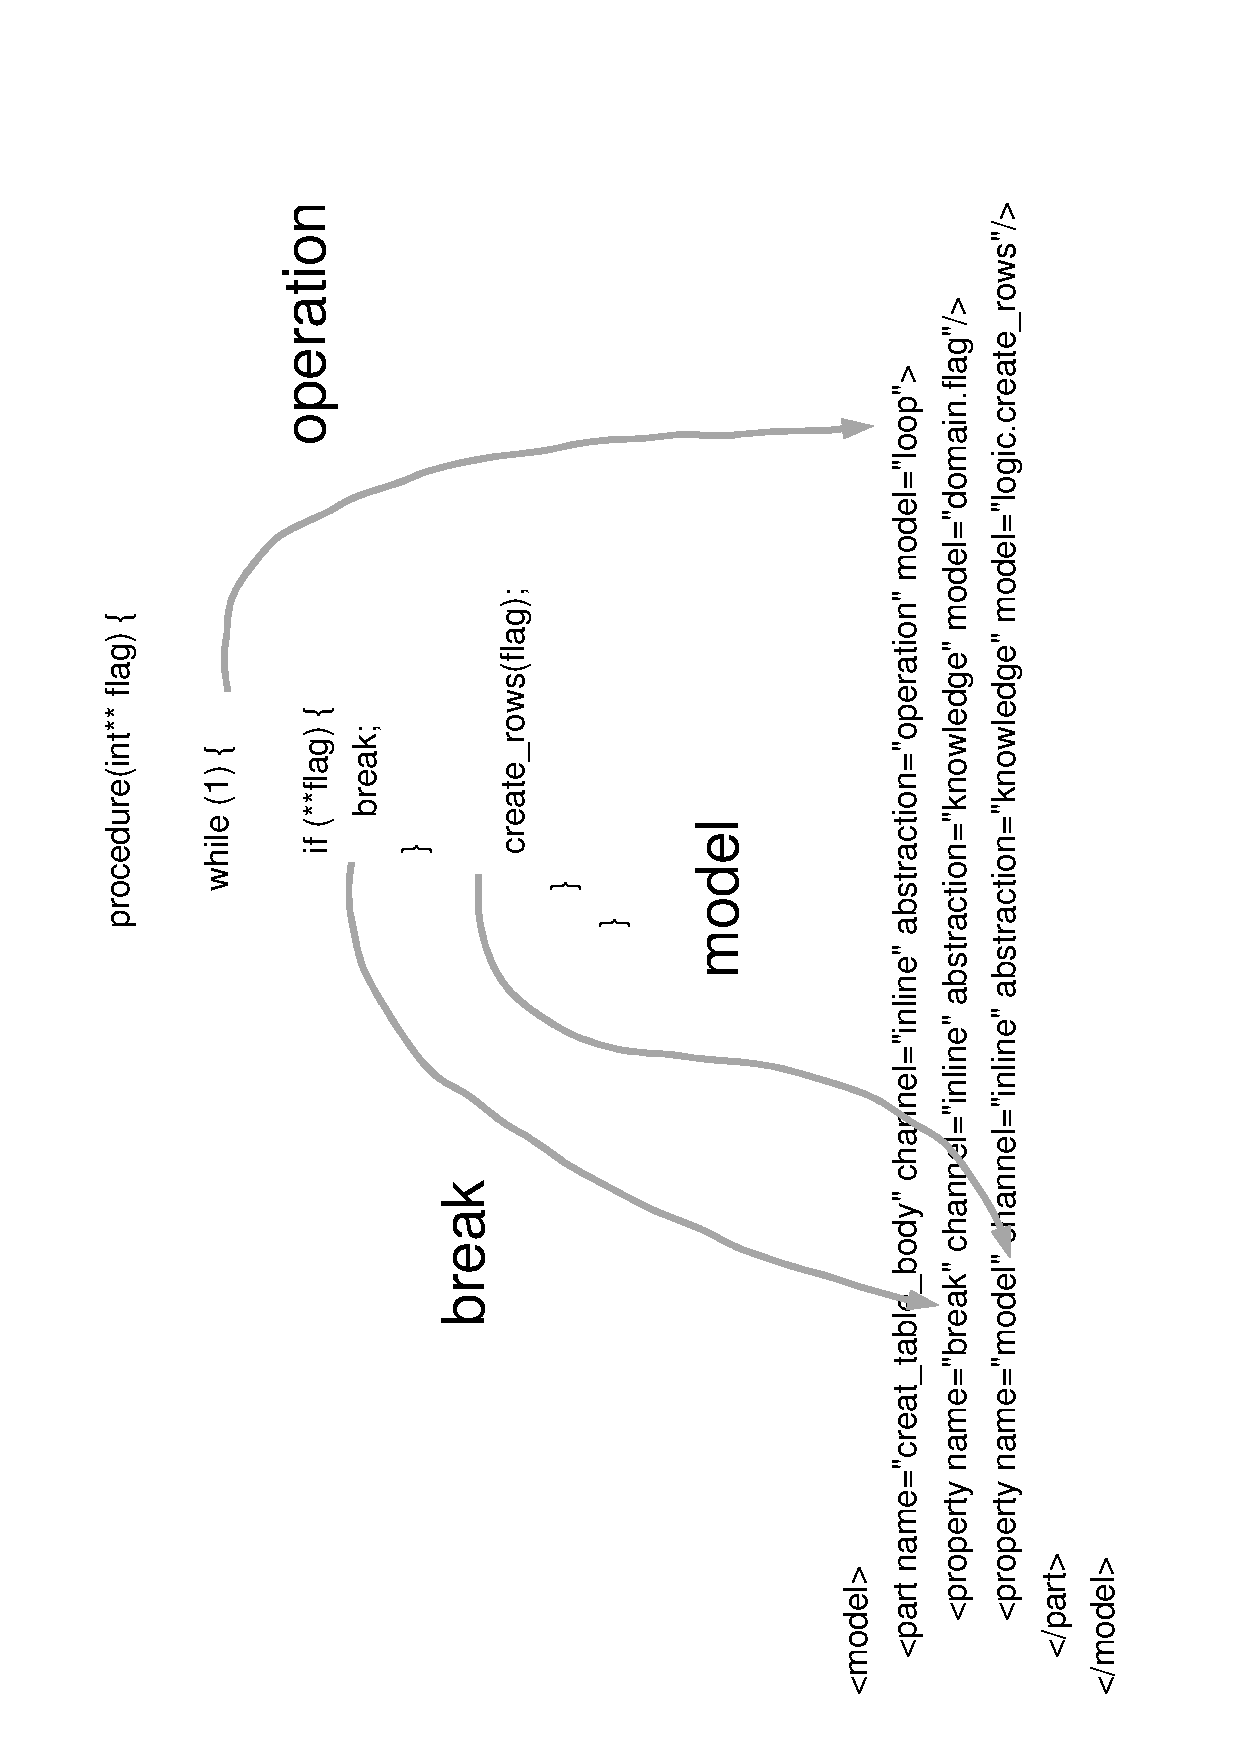
\includegraphics[scale=0.3,angle=-90]{graphics/cybolloop.pdf}
        \caption{Loop Control Structure and Elements in C and CYBOL}
        \label{cybolloop_figure}
    \end{center}
\end{figure}

The \emph{loop} operation needs two parameters to be functional: a \emph{break}
flag as means of interruption and a logic \emph{model} to be executed in each
loop cycle (figure \ref{cybolloop_figure}). An \emph{index} counting loop
cycles is not given, as it is in the responsibility of the logic \emph{model}
to manage that index, just like the setting of the \emph{break} flag,
internally. The following example dynamically creates a table consisting of a
number of rows:

\begin{scriptsize}
    \begin{verbatim}
<model>
    <part name="creat_table_body" channel="inline" abstraction="operation" model="loop">
        <property name="break" channel="inline" abstraction="knowledge" model=".domain.flag"/>
        <property name="model" channel="inline" abstraction="knowledge" model=".logic.create_rows"/>
    </part>
</model>
    \end{verbatim}
\end{scriptsize}

%
% $RCSfile: conditional_execution.tex,v $
%
% Copyright (c) 2002-2007. Christian Heller. All rights reserved.
%
% Permission is granted to copy, distribute and/or modify this document
% under the terms of the GNU Free Documentation License, Version 1.1 or
% any later version published by the Free Software Foundation; with no
% Invariant Sections, with no Front-Cover Texts and with no Back-Cover
% Texts. A copy of the license is included in the section entitled
% "GNU Free Documentation License".
%
% http://www.cybop.net
% - Cybernetics Oriented Programming -
%
% Version: $Revision: 1.1 $ $Date: 2007-08-01 13:59:00 $ $Author: christian $
% Authors: Christian Heller <christian.heller@tuxtax.de>
%

\subsection{Conditional Execution}
\label{conditional_execution_heading}
\index{Conditional Execution Example}

An obviously presupposed part in the previous example is a logic setting the
break \emph{condition} (flag). If the break flag was not set, the loop would
run endlessly. The following knowledge template therefore shows a
\emph{comparison} operation, as it could stand at the end of the loop's logic
model, referenced by the \emph{model} property in the previous example. After
having compared the current loop index with a maximum loop count number, the
break flag may or may not be set. When entering its next cycle, the loop
operation checks whether the flag is set. If so, the loop is stopped:

\begin{scriptsize}
    \begin{verbatim}
<model>
    <part name="comparison" channel="inline" abstraction="operation" model="compare">
        <property name="operator" channel="inline" abstraction="character" model="greater_or_equal"/>
        <property name="left_side" channel="inline" abstraction="knowledge" model=".domain.index"/>
        <property name="right_side" channel="inline" abstraction="knowledge" model=".domain.count"/>
        <property name="result" channel="inline" abstraction="knowledge" model=".domain.flag"/>
    </part>
</model>
    \end{verbatim}
\end{scriptsize}

\begin{figure}[ht]
    \begin{center}
        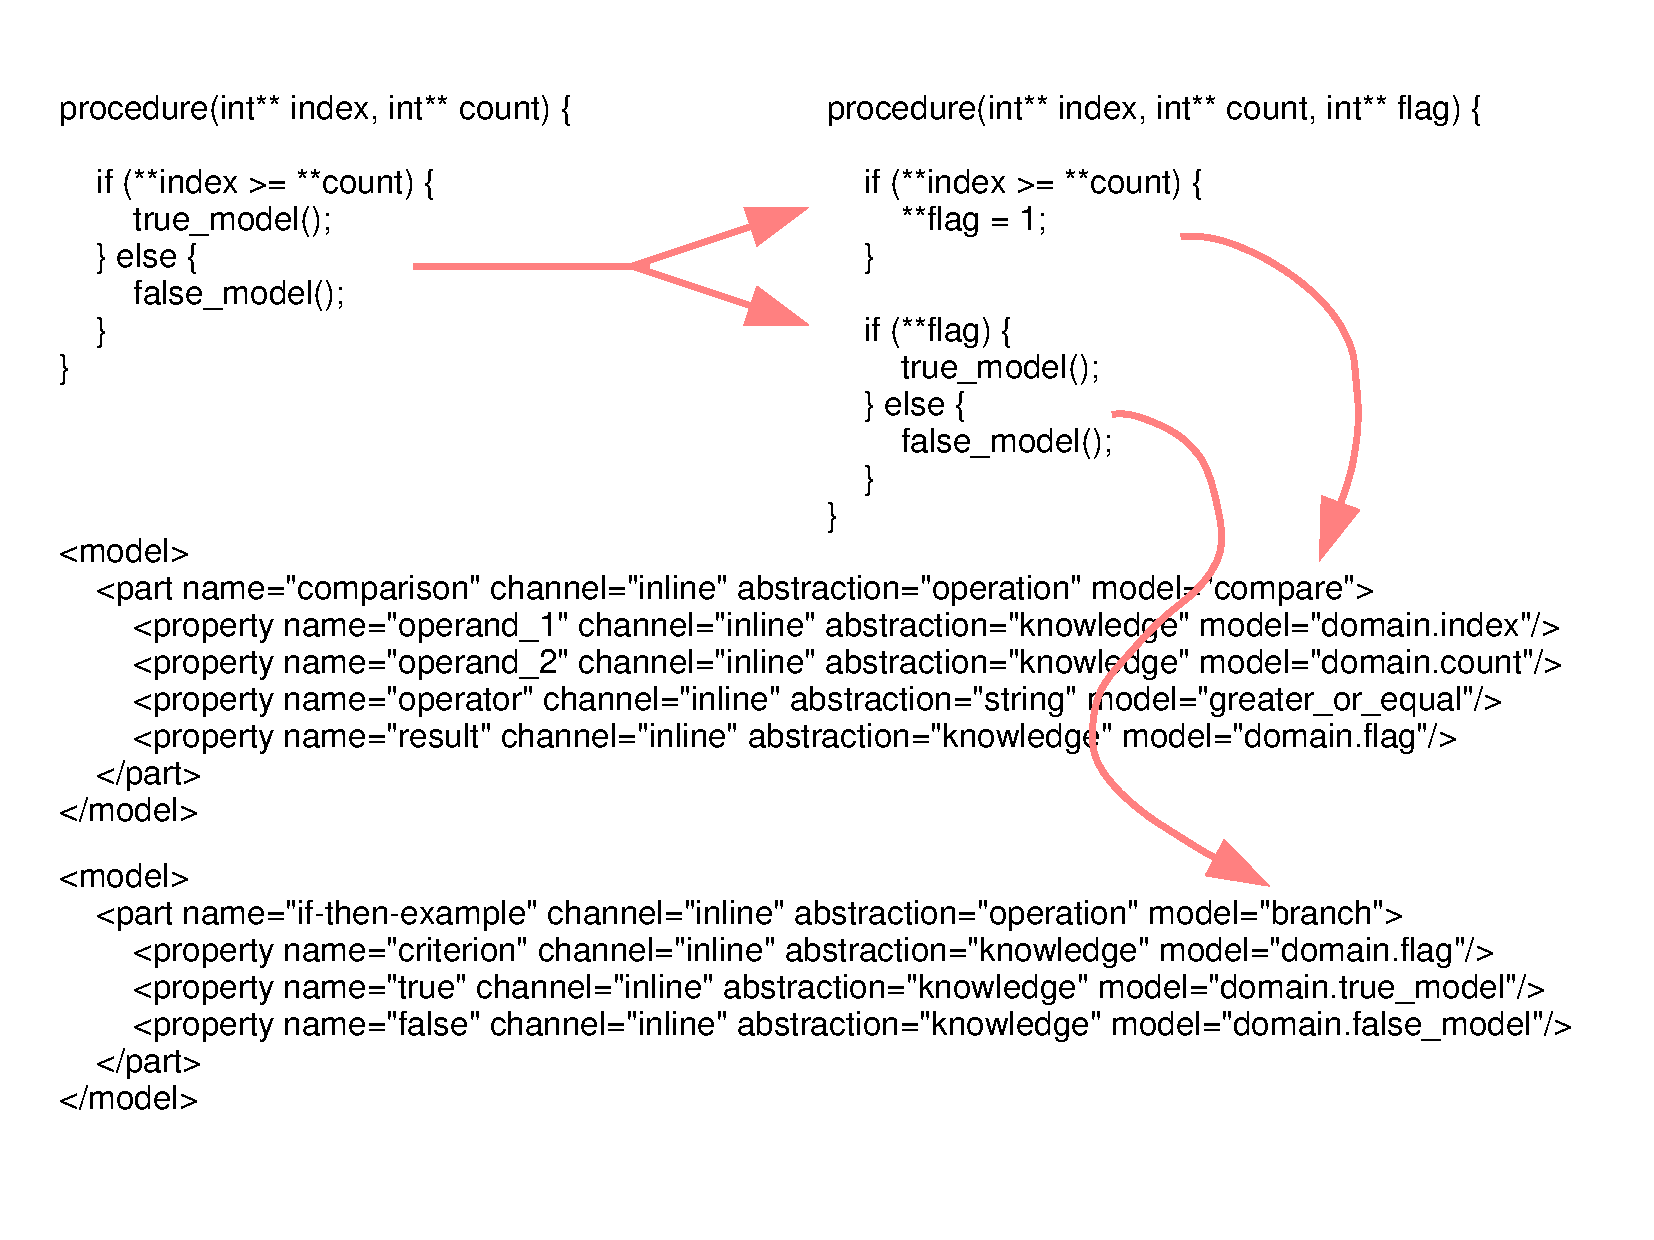
\includegraphics[scale=0.3,angle=-90]{graphics/cybolcondition.pdf}
        \caption{Condition Control Structure and Elements in C and CYBOL}
        \label{cybolcondition_figure}
    \end{center}
\end{figure}

Flags as one of the earliest techniques used in computing (in software as well
as in hardware) are the perfect means for controlling the execution of
primitive logic models, namely operations. They represent a condition set as
result of another logic model -- the latter often being some kind of comparison
operation. In order to execute code upon activation of a flag, a conventional
comparison control structure needs to be split up into two independent blocks
(figure \ref{cybolcondition_figure}), with the flag being the linking element.
The flag which was set by a comparison operation is used for branching the
control flow.

The second example shows how a classical \emph{if-then} statement would be
written in CYBOL. The corresponding operation is called \emph{branch} and it
expects three properties: a \emph{criterion} flag and two models, of which one
is executed in case the flag is \emph{true} and the other is executed otherwise.

\begin{scriptsize}
    \begin{verbatim}
<model>
    <part name="if-then-example" channel="inline" abstraction="operation" model="branch">
        <property name="criterion" channel="inline" abstraction="knowledge" model=".domain.flag"/>
        <property name="true" channel="inline" abstraction="knowledge" model=".domain.true_model"/>
        <property name="false" channel="inline" abstraction="knowledge" model=".domain.false_model"/>
    </part>
</model>
    \end{verbatim}
\end{scriptsize}


%
% $RCSfile: special_examples.tex,v $
%
% Copyright (C) 2002-2008. Christian Heller.
%
% Permission is granted to copy, distribute and/or modify this document
% under the terms of the GNU Free Documentation License, Version 1.1 or
% any later version published by the Free Software Foundation; with no
% Invariant Sections, with no Front-Cover Texts and with no Back-Cover
% Texts. A copy of the license is included in the section entitled
% "GNU Free Documentation License".
%
% http://www.cybop.net
% - Cybernetics Oriented Programming -
%
% http://www.resmedicinae.org
% - Information in Medicine -
%
% Version: $Revision: 1.1 $ $Date: 2008-08-19 20:41:09 $ $Author: christian $
% Authors: Christian Heller <christian.heller@tuxtax.de>
%

\subsection{Special Examples}
\label{special_examples_heading}
\index{CYBOL Special Example Constructs}

\emph{XML} is used for representing data of very different domains, and a whole
plethora of XML dialects exists. Two of them are mentioned following. The main
purpose of the next examples, however, is to show how CYBOL can replace these.

%
% $RCSfile: synchronous_execution.tex,v $
%
% Copyright (c) 2002-2007. Christian Heller. All rights reserved.
%
% Permission is granted to copy, distribute and/or modify this document
% under the terms of the GNU Free Documentation License, Version 1.1 or
% any later version published by the Free Software Foundation; with no
% Invariant Sections, with no Front-Cover Texts and with no Back-Cover
% Texts. A copy of the license is included in the section entitled
% "GNU Free Documentation License".
%
% http://www.cybop.net
% - Cybernetics Oriented Programming -
%
% Version: $Revision: 1.1 $ $Date: 2007-08-01 13:59:00 $ $Author: christian $
% Authors: Christian Heller <christian.heller@tuxtax.de>
%

\subsection{Synchronous Execution}
\label{synchronous_execution_heading}
\index{Synchronous Execution Example}
\index{MusicXML}

\emph{MusicXML} \cite{musicxml} is a markup language \textit{designed to
represent musical scores, specifically common western musical notation from the
17th century onwards.} In principle, CYBOL could be used for this purpose as
well. Of course, there are many details (additional properties) which would
still have to be worked out in order to be able to correctly represent complete
musical scores. As most models, the \emph{Musical Work} displayed in figure
\ref{music_figure} can be considered a hierarchy consisting of \emph{Parts}
(played/ sung by instruments/ voices). Parts in turn consist of
\emph{Measures}, which consist of \emph{Notes}, which finally have a
\emph{Pitch} and sometimes \emph{Lyric}.

\begin{figure}[ht]
    \begin{center}
        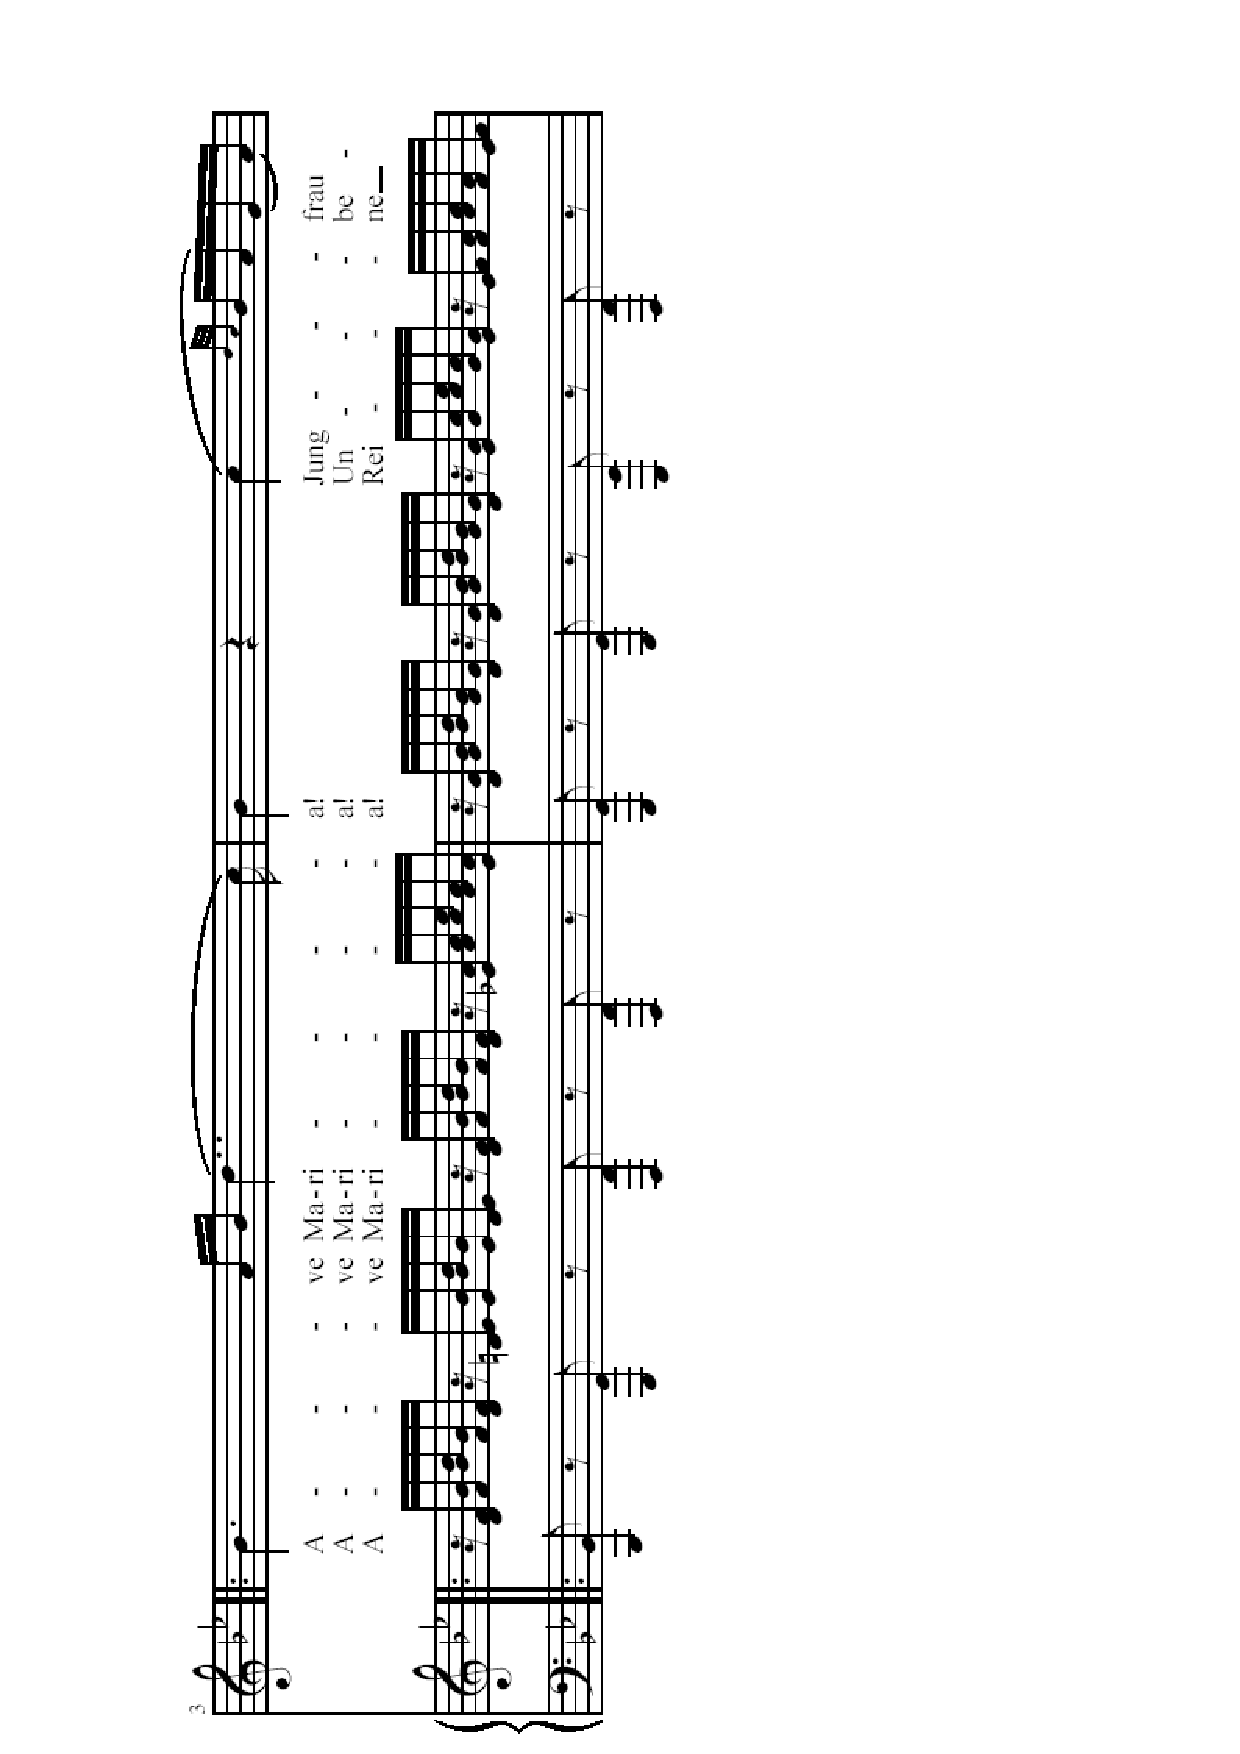
\includegraphics[scale=0.3,angle=-90]{graphics/music.pdf}
%        \caption{Musical Score of Franz Schubert's \emph{Ave Maria} (Ellen's Gesang III) \cite{musicxml}}
        \caption{Musical Score of Franz Schubert's \emph{Ave Maria} \cite{musicxml}}
        \label{music_figure}
    \end{center}
\end{figure}

The following knowledge templates deliver only short examples showing how music
may be modelled in CYBOL. Their property names were taken over from MusicXML's
element tags, as elaborated in \cite{musicxml}. Most are self-explanatory and
shall not be further discussed here. The first example template represents an
extract from a complete musical \emph{Work}, consisting of the two parts
\emph{Voice} and \emph{Piano}:

\begin{scriptsize}
    \begin{verbatim}
<model>
    <part name="number" channel="inline" abstraction="string" model="D. 839"/>
    <part name="title" channel="inline" abstraction="string" model="Ave Maria (Ellen's Gesang III)"/>
    <part name="composer" channel="inline" abstraction="string" model="Franz Schubert"/>
    <part name="poet" channel="inline" abstraction="string" model="Walter Scott"/>
    <part name="voice" channel="file" abstraction="cybol" model="voice.cybol">
        <property name="score_instrument" channel="inline" abstraction="string" model="P1-I14"/>
        <property name="instrument_name" channel="inline" abstraction="string" model="Choir Aahs"/>
        <property name="midi_instrument" channel="inline" abstraction="string" model="P1-I14"/>
        <property name="midi-channel" channel="inline" abstraction="integer" model="1"/>
        <property name="midi-program" channel="inline" abstraction="integer" model="53"/>
    </part>
    <part name="piano" channel="file" abstraction="cybol" model="piano.cybol">
        <property ...
    </part>
</model>
    \end{verbatim}
\end{scriptsize}

One of the \emph{Parts} is shown in the next template. It consists of several measures:

\begin{scriptsize}
    \begin{verbatim}
<model>
    <part name="measure_$1" channel="file" abstraction="cybol" model="measure_1.cybol">
        <property name="divisions" channel="inline" abstraction="integer" model="48"/>
        <property name="key_fifths" channel="inline" abstraction="integer" model="-2"/>
        <property name="key_mode" channel="inline" abstraction="string" model="major"/>
        <property name="beats" channel="inline" abstraction="integer" model="4"/>
        <property name="beat_type" channel="inline" abstraction="integer" model="4"/>
        <property name="staves" channel="inline" abstraction="integer" model="0"/>
        <property name="clef_sign" channel="inline" abstraction="string" model="G"/>
        <property name="clef_line" channel="inline" abstraction="integer" model="2"/>
    </part>
    <part name="measure_$2" channel="file" abstraction="cybol" model="measure_2.cybol">
        <property ...
    </part>
</model>
    \end{verbatim}
\end{scriptsize}

A \emph{Measure} again consists of \emph{Notes}:

\begin{scriptsize}
    \begin{verbatim}
<model>
    <part name="note_$1" channel="file" abstraction="cybol" model="note_1.cybol">
        <property name="duration" channel="inline" abstraction="integer" model="72"/>
        <property name="voice" channel="inline" abstraction="integer" model="1"/>
        <property name="type" channel="inline" abstraction="string" model="quarter"/>
        <property name="stem" channel="inline" abstraction="string" model="down"/>
        <property name="position" channel="inline" abstraction="integer" model="1"/>
    </part>
    <part name="note_$2" channel="file" abstraction="cybol" model="note_2.cybol">
        <property name="duration" channel="inline" abstraction="integer" model="12"/>
        <property name="voice" channel="inline" abstraction="integer" model="1"/>
        <property name="type" channel="inline" abstraction="string" model="16th"/>
        <property name="stem" channel="inline" abstraction="string" model="up"/>
        <property name="position" channel="inline" abstraction="integer" model="2"/>
    </part>
    <part name="note_$3" channel="file" abstraction="cybol" model="note_3.cybol">
        <property ...
        <property name="position" channel="inline" abstraction="integer" model="2"/>
    </part>
</model>
    \end{verbatim}
\end{scriptsize}

An important property to note here is the \emph{position} value. It is common
that two notes have to be played at the same time, the notes then being called
a \emph{Chord}. In contrast to MusicXML which provides an own tag to denote
notes belonging to the same chord, CYBOL suggests to use a \emph{position}
property having identical values for all notes in a chord. An interpreter
program may thus not only read necessary sequence information, but can also
figure out which of the notes have to be played \emph{synchronously}.

A fourth example represents one \emph{Note}, consisting of a \emph{Pitch} and
\emph{Lyric} text, which are the final abstractions in this knowledge template:

\begin{scriptsize}
    \begin{verbatim}
<model>
    <part name="pitch" channel="inline" abstraction="string" model="B">
        <property name="alter" channel="inline" abstraction="integer" model="-1"/>
        <property name="octave" channel="inline" abstraction="integer" model="4"/>
    </part>
    <part name="lyric" channel="inline" abstraction="string" model="A">
        <property name="syllabic" channel="inline" abstraction="string" model="begin"/>
    </part>
</model>
    \end{verbatim}
\end{scriptsize}

%
% $RCSfile: presentation_and_content.tex,v $
%
% Copyright (c) 2002-2007. Christian Heller. All rights reserved.
%
% Permission is granted to copy, distribute and/or modify this document
% under the terms of the GNU Free Documentation License, Version 1.1 or
% any later version published by the Free Software Foundation; with no
% Invariant Sections, with no Front-Cover Texts and with no Back-Cover
% Texts. A copy of the license is included in the section entitled
% "GNU Free Documentation License".
%
% http://www.cybop.net
% - Cybernetics Oriented Programming -
%
% Version: $Revision: 1.1 $ $Date: 2007-08-01 13:59:00 $ $Author: christian $
% Authors: Christian Heller <christian.heller@tuxtax.de>
%

\subsection{Presentation and Content}
\label{presentation_and_content_heading}
\index{Presentation and Content Example}
\index{Mathematical Markup Language}
\index{MathML}

The \emph{Mathematical Markup Language} (MathML) \cite{mathml} provides means
for representing mathematical expressions, that is \emph{Content} as well as
\emph{Presentation} of data. Both are discrete models, comparable to the
\emph{Domain} and \emph{User Interface} (UI) of a software application, which
can be translated into each other.

CYBOL uses just four tags (section \ref{semantics_heading}) but can represent
mathematical expressions as well. What MathML calls \emph{Content}, becomes a
\emph{Logic} knowledge template in CYBOL. The mathematical content of the
formula $(a + b)^{2}$ would be modelled as follows:

\begin{scriptsize}
    \begin{verbatim}
<model>
    <part name="addition" channel="inline" abstraction="operation" model="add">
        <property name="abstraction" channel="inline" abstraction="character" model="integer"/>
        <property name="summand_1" channel="inline" abstraction="knowledge" model=".domain.a"/>
        <property name="summand_2" channel="inline" abstraction="knowledge" model=".domain.b"/>
        <property name="sum" channel="inline" abstraction="knowledge" model=".domain.c"/>
    </part>
    <part name="exponentiation" channel="inline" abstraction="operation" model="power">
        <property name="base" channel="inline" abstraction="knowledge" model=".domain.c"/>
        <property name="power" channel="inline" abstraction="integer" model="2"/>
        <property name="result" channel="inline" abstraction="knowledge" model=".domain.r"/>
    </part>
</model>
    \end{verbatim}
\end{scriptsize}

And the formula's \emph{Presentation} would be defined by the following two
CYBOL \emph{State} knowledge templates, of which the second one represents the
\emph{Base} that is referenced by the first one:

\begin{scriptsize}
    \begin{verbatim}
<model>
    <part name="base" channel="file" abstraction="compound" model="domain/base.cybol">
        <property name="fence" channel="inline" abstraction="boolean" model="true"/>
    </part>
    <part name="power" channel="inline" abstraction="integer" model="2">
        <property name="superscript" channel="inline" abstraction="boolean" model="true"/>
    </part>
</model>

<model>
    <part name="summand_$1" channel="inline" abstraction="character" model="a"/>
    <part name="operator" channel="inline" abstraction="character" model="+"/>
    <part name="summand_$2" channel="inline" abstraction="character" model="b"/>
</model>
    \end{verbatim}
\end{scriptsize}

%
% $RCSfile: hello_world.tex,v $
%
% Copyright (c) 2005-2006. Christian Heller. All rights reserved.
%
% Permission is granted to copy, distribute and/or modify this document
% under the terms of the GNU Free Documentation License, Version 1.1 or
% any later version published by the Free Software Foundation; with no
% Invariant Sections, with no Front-Cover Texts and with no Back-Cover
% Texts. A copy of the license is included in the section entitled
% "GNU Free Documentation License".
%
% http://www.cybop.net
% - Cybernetics Oriented Programming -
%
% http://www.resmedicinae.org
% - Information in Medicine -
%
% Version: $Revision: 1.1 $ $Date: 2006-01-03 08:21:45 $ $Author: christian $
% Authors: Christian Heller <christian.heller@tuxtax.de>
%

\subsection{Hello World}
\label{hello_world_heading}

The well-known \emph{Hello, World!} program printing just two words shall be
given as minimal example application. It consists of only two operations:
\emph{send} and \emph{exit}. The string message to be displayed on screen is
handed over as \emph{property} to the \emph{send} operation, before the
\emph{exit} shuts down the system:

\begin{scriptsize}
    \begin{verbatim}
<model>
    <part name="send_model_to_output"
        channel="inline"
        abstraction="operation"
        model="send">
        <property name="language"
            channel="inline"
            abstraction="string"
            model="tui"/>
        <property name="receiver"
            channel="inline"
            abstraction="string"
            model="user"/>
        <property name="message"
            channel="inline"
            abstraction="string"
            model="Hello, World!"/>
    </part>
    <part name="exit_application"
        channel="inline"
        abstraction="operation"
        model="exit"/>
</model>
    \end{verbatim}
\end{scriptsize}

%
% $RCSfile: any_system.tex,v $
%
% Copyright (C) 2002-2008. Christian Heller.
%
% Permission is granted to copy, distribute and/or modify this document
% under the terms of the GNU Free Documentation License, Version 1.1 or
% any later version published by the Free Software Foundation; with no
% Invariant Sections, with no Front-Cover Texts and with no Back-Cover
% Texts. A copy of the license is included in the section entitled
% "GNU Free Documentation License".
%
% http://www.cybop.net
% - Cybernetics Oriented Programming -
%
% http://www.resmedicinae.org
% - Information in Medicine -
%
% Version: $Revision: 1.1 $ $Date: 2008-08-19 20:41:05 $ $Author: christian $
% Authors: Christian Heller <christian.heller@tuxtax.de>
%

\subsubsection{Any System?}
\label{any_system_heading}
\index{CYBOL for Any System}

While creating the CYBOP knowledge concepts and implementing them in the CYBOL
language, one main aim was to make that language as flexible as possible, in
order to be usable for the development of a variety of systems. It seems that
CYBOL is indeed applicable for developing standard business applications in
very different domains.

It might also be usable for creating desktop environments such as the
\emph{K Desktop Environment} (KDE) \cite{kde} -- and even configuration parts
of an \emph{Operating System} (OS) (the information stored in the files of the
\emph{/etc} directory and the \emph{/usr/src/linux/.config} file, when taking
the Linux kernel as example) could possibly be encoded in CYBOL. The same
counts for the configuration files of applications residing in the \emph{/etc}
directory of systems that follow the \emph{Filesystem Hierarchy Standard}
(FHS). That is, both applications and their configuration files may be written
in the same format: CYBOL.

Yet to limit the scope of this work, proof for these assumptions cannot be
given here. As well, the applicability of CYBOL for programming \emph{Real Time}
(RT) systems was not investigated yet. A slightly more extensive example,
however, is given in chapter \ref{res_medicinae_heading}, which describes the
\emph{Res Medicinae} prototype -- a yet very incomplete
\emph{Electronic Health Record} (EHR) application.


%
% $RCSfile: inheritance_as_property.tex,v $
%
% Copyright (c) 2002-2007. Christian Heller. All rights reserved.
%
% Permission is granted to copy, distribute and/or modify this document
% under the terms of the GNU Free Documentation License, Version 1.1 or
% any later version published by the Free Software Foundation; with no
% Invariant Sections, with no Front-Cover Texts and with no Back-Cover
% Texts. A copy of the license is included in the section entitled
% "GNU Free Documentation License".
%
% http://www.cybop.net
% - Cybernetics Oriented Programming -
%
% Version: $Revision: 1.1 $ $Date: 2007-08-01 13:59:00 $ $Author: christian $
% Authors: Christian Heller <christian.heller@tuxtax.de>
%

\section{Inheritance as Property}
\label{inheritance_as_property_heading}
\index{Inheritance as CYBOL Property}

One fundamental concept of \emph{Object Oriented Programming} (OOP) is
\emph{Inheritance}. In principle, there is no problem with implementing
inheritance in CYBOL. If done, however, it would differ from traditional class
architectures as known from OOP. Classical OOP systems resolve inheritance
relationships at runtime; CYBOP systems, on the other hand, would resolve them
just once when creating a knowledge model (instance) from a knowledge template.
After instantiation, all inheritance relationships are lost since instances are
stored as purely hierarchical \emph{whole}-\emph{part} models in memory,
without any links to \emph{super} models.

The following knowledge template shows how inheritance could be realised in
CYBOL. Contrary to OOP classes which hold a link to their corresponding
\emph{super} class as \emph{intrinsic} property, a CYBOL knowledge template
does not know itself from which \emph{super} template to inherit from. That
information is stored as \emph{extrinsic} property outside the template
instead, in other words in the \emph{whole} template to which the inheriting
template belongs.

\begin{scriptsize}
    \begin{verbatim}
<model>
    <part name="ok_button" channel="file" abstraction="cybol" model="gui/ok_button.cybol">
        <property name="super" channel="file" abstraction="cybol" model="button.cybol"/>
        <property name="size" channel="inline" abstraction="integer" model="90,30,1"/>
        <property name="colour" channel="inline" abstraction="rgb" model="127,127,127"/>
    </part>
</model>
    \end{verbatim}
\end{scriptsize}

One of the properties in the example template above carries the name
\emph{super}. Its model references another template which is treated as super
template of the corresponding \emph{part} the property belongs to. With slight
modifications on the property name \emph{super}, which has to be unique among
all properties of a part, it would even be possible to implement
\emph{Multiple Inheritance}. Dependency complications are not to be expected
because all inheritance relationships are forgotten in runtime models.

Although the described inheritance mechanism was tested successfully in an
older prototype application, it has not been implemented in CYBOL. None of the
created example applications showed a need for it, nor did any of them promise
more effective programming. The reuse of CYBOL templates is realised through
composition only, that is fine-granular templates make up more coarse-grained
ones. This counts for both, state- as well as logic models, since they are not
bundled like in OOP. And polymorphism as effect does not have to be considered.

%
% $RCSfile: container_mapping.tex,v $
%
% Copyright (c) 2002-2007. Christian Heller. All rights reserved.
%
% Permission is granted to copy, distribute and/or modify this document
% under the terms of the GNU Free Documentation License, Version 1.1 or
% any later version published by the Free Software Foundation; with no
% Invariant Sections, with no Front-Cover Texts and with no Back-Cover
% Texts. A copy of the license is included in the section entitled
% "GNU Free Documentation License".
%
% http://www.cybop.net
% - Cybernetics Oriented Programming -
%
% Version: $Revision: 1.1 $ $Date: 2007-08-01 13:59:00 $ $Author: christian $
% Authors: Christian Heller <christian.heller@tuxtax.de>
%

\section{Container Mapping}
\label{container_mapping_heading}
\index{Containers in CYBOL}
\index{Mapping Containers to CYBOL}

State-of-the-art programming languages like Java offer a number of different
container types (figure \ref{container_figure}).

\begin{figure}[ht]
    \begin{center}
        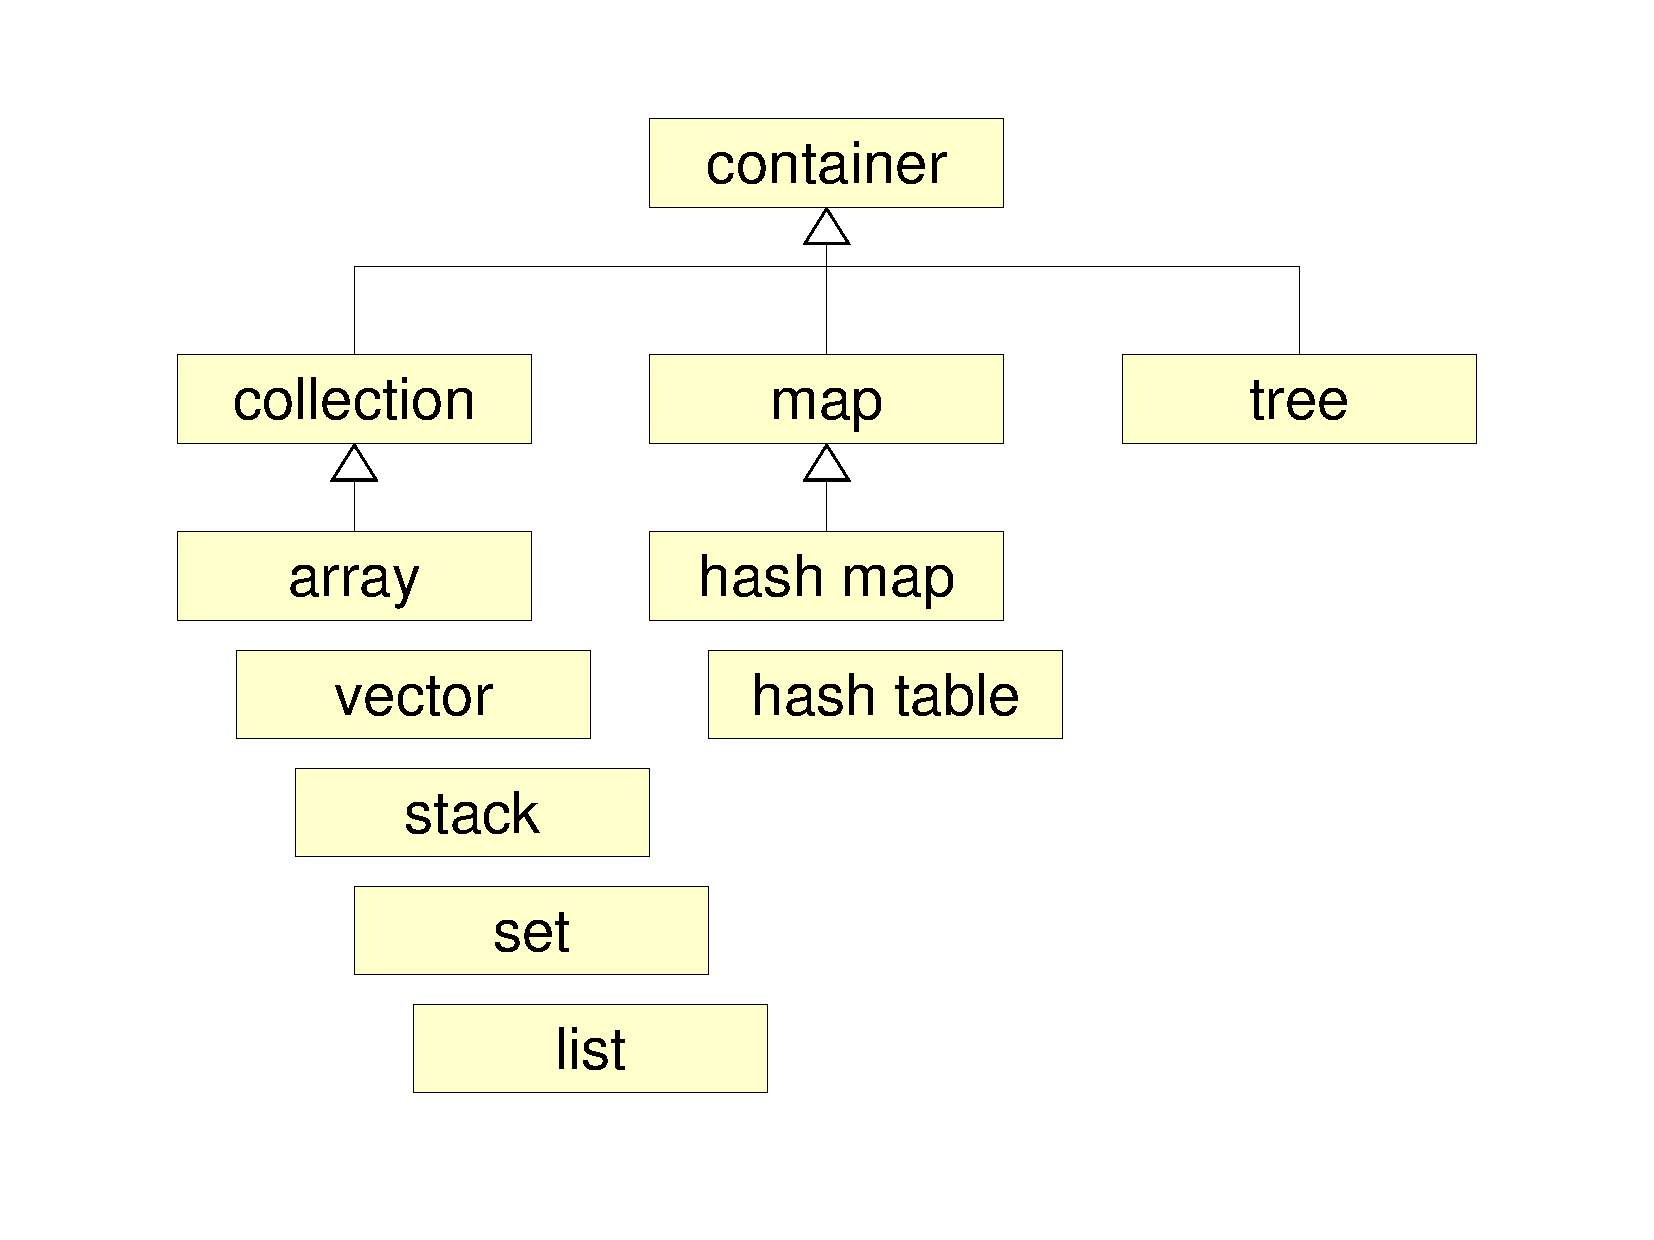
\includegraphics[scale=0.3,angle=-90]{graphics/container.pdf}
        \caption{Classical Container Types in Java}
        \label{container_figure}
    \end{center}
\end{figure}

\begin{table}[ht]
    \begin{center}
        \begin{footnotesize}
        \begin{tabular}{| p{35mm} | p{70mm} |}
            \hline
            \textbf{Classical Container Type} & \textbf{Realisation in CYBOL Knowledge Template}\\
            \hline
            Tree & Hierarchical \emph{whole}-\emph{part} structure\\
            \hline
            Table & Like a Tree, as hierarchy consisting of rows which consist of columns\\
            \hline
            Map & Parts have a \emph{name} (key) and a \emph{model} (value)\\
            \hline
            List & Parts may have a \emph{position} property\\
            \hline
            Vector & A \emph{model} attribute may hold comma-separated values;
                an extra template holds a dynamically changeable number of parts\\
            \hline
            Array & Like a Vector; characters are interpreted as \emph{string}\\
            \hline
        \end{tabular}
        \end{footnotesize}
        \caption{Mapping Classical Containers to CYBOL}
        \label{mapping_table}
    \end{center}
\end{table}

CYBOI owns a \emph{Knowledge Schema} which represents each item as
\emph{Hierarchy} by default, the result being that different types of
containers are \emph{not} needed any longer, that is are unified. Table
\ref{mapping_table} shows how the different kinds of container behaviour are
implemented in CYBOL. As can be seen, CYBOL is able to represent many container
types.

%
% $RCSfile: hidden_patterns.tex,v $
%
% Copyright (c) 2002-2007. Christian Heller. All rights reserved.
%
% Permission is granted to copy, distribute and/or modify this document
% under the terms of the GNU Free Documentation License, Version 1.1 or
% any later version published by the Free Software Foundation; with no
% Invariant Sections, with no Front-Cover Texts and with no Back-Cover
% Texts. A copy of the license is included in the section entitled
% "GNU Free Documentation License".
%
% http://www.cybop.net
% - Cybernetics Oriented Programming -
%
% Version: $Revision: 1.1 $ $Date: 2007-08-01 13:59:00 $ $Author: christian $
% Authors: Christian Heller <christian.heller@tuxtax.de>
%

\section{Hidden Patterns}
\label{hidden_patterns_heading}
\index{Patterns in CYBOL}
\index{Hidden Patterns in CYBOL}

There are a number of software patterns that may not be obvious (hidden) at
first sight, but have been considered in the design of the CYBOL language.

Most obviously, CYBOL knowledge templates follow the \emph{Composite} pattern,
in a simplified form. All templates represent a compound consisting of part
templates, which leads to a tree-like structure. But this also means that related
patterns like \emph{Whole-Part} and \emph{Wrapper} are representable by CYBOL
knowledge templates. A template as whole wraps its parts.

Knowledge templates with similar granularity can be collected in one directory,
in other words one common ontological level. Templates with smaller granularity,
that is those that the more coarse-grained templates consist of, can be placed
in another common layer and so forth. What comes out of it is a system of levels
-- one variant of the \emph{Layers} pattern.


%
% $RCSfile: comparison.tex,v $
%
% Copyright (c) 2002-2007. Christian Heller. All rights reserved.
%
% Permission is granted to copy, distribute and/or modify this document
% under the terms of the GNU Free Documentation License, Version 1.1 or
% any later version published by the Free Software Foundation; with no
% Invariant Sections, with no Front-Cover Texts and with no Back-Cover
% Texts. A copy of the license is included in the section entitled
% "GNU Free Documentation License".
%
% http://www.cybop.net
% - Cybernetics Oriented Programming -
%
% Version: $Revision: 1.1 $ $Date: 2007-07-17 20:02:36 $ $Author: christian $
% Authors: Christian Heller <christian.heller@tuxtax.de>
%

\section{Comparison}
\label{comparison_heading}
\index{Comparison}

%
% $RCSfile: compare.tex,v $
%
% Copyright (c) 2002-2007. Christian Heller. All rights reserved.
%
% Permission is granted to copy, distribute and/or modify this document
% under the terms of the GNU Free Documentation License, Version 1.1 or
% any later version published by the Free Software Foundation; with no
% Invariant Sections, with no Front-Cover Texts and with no Back-Cover
% Texts. A copy of the license is included in the section entitled
% "GNU Free Documentation License".
%
% http://www.cybop.net
% - Cybernetics Oriented Programming -
%
% Version: $Revision: 1.1 $ $Date: 2007-07-17 20:02:36 $ $Author: christian $
% Authors: Christian Heller <christian.heller@tuxtax.de>
%

\subsection{Compare}
\label{compare_heading}
\index{Compare}

This operation compares two given operands.

\subsubsection{Comparison Property}

\emph{required}

name=\texttt{'comparison'}\\
abstraction=\texttt{'character'}\\
model=\texttt{'equal' \vline\ 'smaller' \vline\ 'greater' \vline\ 'smaller\_or\_equal' \vline\ 'greater\_or\_equal'}

This is the kind of comparison to be applied.

\subsubsection{Left Side Property}

\emph{required}

name=\texttt{'left\_side'}\\
abstraction=\texttt{'boolean' \vline\ 'integer' \vline\ 'float' \vline\ 'character' \vline\ 'knowledge' \vline\ 'encapsulated'}\\
model=\texttt{value or knowledge model}

This is the left side value of the comparison.

\subsubsection{Right Side Property}

\emph{required}

name=\texttt{'right\_side'}\\
abstraction=\texttt{'boolean' \vline\ 'integer' \vline\ 'float' \vline\ 'character' \vline\ 'knowledge' \vline\ 'encapsulated'}\\
model=\texttt{value or knowledge model}

This is the right side value of the comparison.

\subsubsection{Result Property}

\emph{required}

name=\texttt{'result'}\\
abstraction=\texttt{'boolean' \vline\ 'knowledge' \vline\ 'encapsulated'}\\
model=\texttt{result knowledge model}

This is the knowledge model in which the comparison result is stored.

\subsubsection{Selection Property}

\emph{optional}, only if comparing values of abstraction "character"

name=\texttt{'selection'}\\
abstraction=\texttt{'character'}\\
model=\texttt{'full' \vline\ 'prefix' \vline\ 'suffix' \vline\ 'part'}

This property selects which part of two string values shall be compared.


%
% $RCSfile: tool_support.tex,v $
%
% Copyright (C) 2002-2008. Christian Heller.
%
% Permission is granted to copy, distribute and/or modify this document
% under the terms of the GNU Free Documentation License, Version 1.1 or
% any later version published by the Free Software Foundation; with no
% Invariant Sections, with no Front-Cover Texts and with no Back-Cover
% Texts. A copy of the license is included in the section entitled
% "GNU Free Documentation License".
%
% http://www.cybop.net
% - Cybernetics Oriented Programming -
%
% http://www.resmedicinae.org
% - Information in Medicine -
%
% Version: $Revision: 1.1 $ $Date: 2008-08-19 20:41:09 $ $Author: christian $
% Authors: Christian Heller <christian.heller@tuxtax.de>
%

\section{Tool Support}
\label{tool_support_heading}
\index{CYBOL Tool Support}

When proposing a new theory of computing, or a new programming language, it is
common to provide a suitable \emph{Integrated Development Environment} (IDE)
supporting the application of that theory or language. If not the tools
themselves, a recommendation for how they may look like should be given at
least. This is what the following sections try to achieve.

%
% $RCSfile: template_editor.tex,v $
%
% Copyright (C) 2002-2008. Christian Heller.
%
% Permission is granted to copy, distribute and/or modify this document
% under the terms of the GNU Free Documentation License, Version 1.1 or
% any later version published by the Free Software Foundation; with no
% Invariant Sections, with no Front-Cover Texts and with no Back-Cover
% Texts. A copy of the license is included in the section entitled
% "GNU Free Documentation License".
%
% http://www.cybop.net
% - Cybernetics Oriented Programming -
%
% http://www.resmedicinae.org
% - Information in Medicine -
%
% Version: $Revision: 1.1 $ $Date: 2008-08-19 20:41:09 $ $Author: christian $
% Authors: Christian Heller <christian.heller@tuxtax.de>
%

\subsection{Template Editor}
\label{template_editor_heading}
\index{CYBOL Template Editor}
\index{Triple-Choice CYBOL Template Editor}

CYBOL applications can be written in an XML-conform way. The use of standard
XML tools to edit and validate CYBOL knowledge templates, at design time, is
therefore possible. An exception are serialised runtime CYBOL models, possibly
made persistent in form of files or in a \emph{Database} (DB), for which XML
conformity has to be given up due to additional markup tokens, as explained in
section \ref{serialised_model_heading}.

Due to the fixed structure of CYBOL knowledge templates (four XML tags, four
XML attributes), more convenient- than standard XML editors shall be
providable. Figure \ref{editor_figure} shows an editor proposal supporting
both, the \emph{Whole-Part-} as well as the \emph{Meta Hierarchy} of CYBOL.
There are three characters indicating the action that a click on a tree node
would evoke:

\begin{itemize}
    \item[+] Open the whole-part hierarchy
    \item[\&] Open the meta hierarchy (properties and constraints)
    \item[-] Close the hierarchy
\end{itemize}

\begin{figure}[ht]
    \begin{center}
        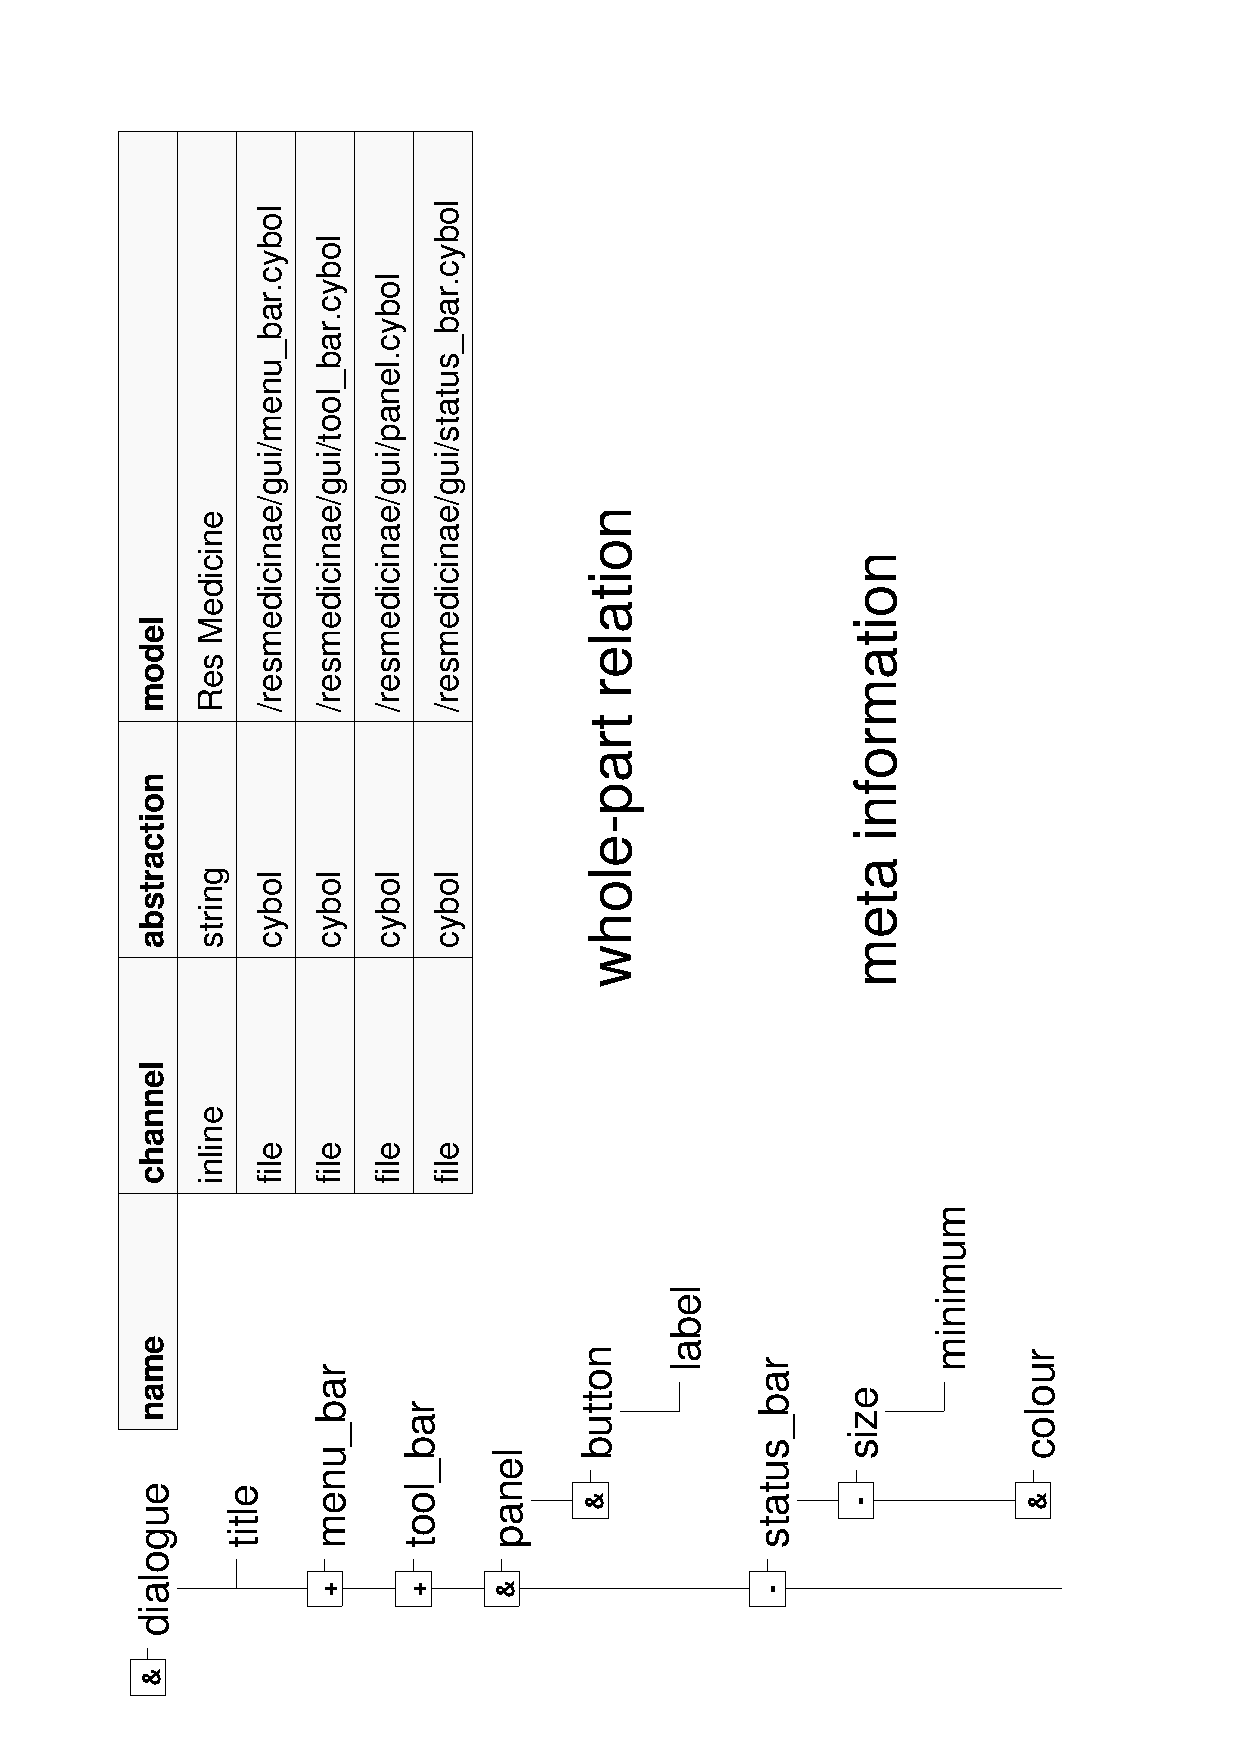
\includegraphics[scale=0.3,angle=-90]{graphic/editor.pdf}
        \caption{CYBOL Editor Supporting Double Hierarchies by Triple Choice}
        \label{editor_figure}
    \end{center}
\end{figure}

The displayed template represents a graphical \emph{dialogue} with its
\emph{title}, \emph{menubar}, \emph{toolbar}, \emph{panel} and \emph{status bar}.
The opened panel node shows its parts, namely \emph{button} and \emph{label}.
The opened status bar node, on the other hand, shows its properties \emph{size}
and \emph{colour}, and additionally the \emph{size}'s \emph{minimum} constraint.
The attribute values of a selected node would be editable in a table like the
one shown on the right-hand side of the figure.

%Prot?g? is an ontology editor and a knowledge-base editor.
%http://protege.stanford.edu/

%
% $RCSfile: knowledge_designer.tex,v $
%
% Copyright (C) 2002-2008. Christian Heller.
%
% Permission is granted to copy, distribute and/or modify this document
% under the terms of the GNU Free Documentation License, Version 1.1 or
% any later version published by the Free Software Foundation; with no
% Invariant Sections, with no Front-Cover Texts and with no Back-Cover
% Texts. A copy of the license is included in the section entitled
% "GNU Free Documentation License".
%
% http://www.cybop.net
% - Cybernetics Oriented Programming -
%
% http://www.resmedicinae.org
% - Information in Medicine -
%
% Version: $Revision: 1.1 $ $Date: 2008-08-19 20:41:07 $ $Author: christian $
% Authors: Christian Heller <christian.heller@tuxtax.de>
%

\subsection{Knowledge Designer}
\label{knowledge_designer_heading}
\index{CYBOL Knowledge Designer}
\index{Unified Modeling Language}
\index{UML}
\index{CYBOL Template Diagram}
\index{TD}
\index{CYBOL Model Diagram}
\index{MD}
\index{CYBOL Organisation Diagram}
\index{OD}
\index{CYBOL Communication Diagram}
\index{CD}

Section \ref{unified_modeling_language_heading} classified diagrams of the
\emph{Unified Modeling Language} (UML) notation into \emph{Structure},
\emph{Behaviour} and \emph{Interaction}. With interaction- being a subset of
behaviour diagrams, there are actually just \emph{two} main categories for UML
diagram classification: \emph{Structure} and \emph{Behaviour}. Since the idea
underlying \emph{this} work is to look at systems from two perspectives
(section \ref{approach_heading}): \emph{Statics} and \emph{Dynamics}, whereby
the former gets split up into two further perspectives: \emph{States} and
\emph{Logic}, the question arises whether or not UML diagrams could be
categorised accordingly? The answer is: \emph{Not quite.} There are a number of
aspects that have to be considered:

\begin{itemize}
    \item[-] UML classes bundle state- and logic aspects (attributes and
        methods). A CsD does not only express the relations between attributes,
        but also those between methods. This fact makes it impossible to sort
        that diagram into just one of the categories: state or logic. Likewise
        does an SD, to take a second example, not just display the order of
        message calls, but also their bundling with objects. CYBOL templates,
        on the other hand, strictly separate state- and logic knowledge.
    \item[-] Classes in a CsD are linked network-like and may have bidirectional
        relations. Composition (recursion) as concept is missing in the class
        element of the UML meta model. The CYBOP knowledge schema is innately
        hierarchical and uses solely unidirectional relations.
    \item[-] UML objects (instances) know from which class (type) they stem from.
        Not at least, this is necessary for mechanisms like polymorphism (based
        on runtime inheritance) to work. CYBOL models know nothing about the
        original template they were initialised with; any links to it are lost.
\end{itemize}

However, an attempt will now be made to categorise the UML diagrams accordingly:

\begin{itemize}
    \item \emph{Statics (States):} CsD
    \item \emph{Statics (Logic):} SMD, AD, SD, TiD, CoD, IOD, UCD
    \item \emph{Dynamics:} ObD, CSD
    \item \emph{Others:} CmD, PD, DD
\end{itemize}

All diagrams formerly belonging to either \emph{Behaviour} or \emph{Interaction},
are now summed up in the \emph{Statics (Logic)} category. Former \emph{Structure}
diagrams are split up into the one describing \emph{Statics (States)} and those
illustrating \emph{Dynamics} (runtime aspects). Some diagrams dealing with issues
like packaging or distribution are put into an extra category called \emph{Others}.

Because of the different programming philosophy behind CYBOP, standard UML
diagrams cannot be used unalteredly for the design of CYBOL applications. Some
of them, however, could be quite useful, when adapted a bit. The \emph{Importance}
column in table \ref{diagrams_table} indicated that not all diagram types are
really needed to effectively design a system. For creating CYBOL applications,
the following four can be considered sufficient. They model the structure of:

\begin{enumerate}
    \item \emph{Template Diagram} (TD): one design-time template (hierarchical,
        ontological concept), with purely unidirectional relations; does not
        illustrate relations between different concepts, as these are only
        established by logic models at runtime; could look like CsD or a tree,
        only that a template may not only represent states, but also logic
        (algorithms, workflows) (figure \ref{td_figure})
    \item \emph{Model Diagram} (MD): the runtime model tree; comparable to ObD,
        but a simple tree with named nodes would suffice; is important because
        input/ output parameters of operations are given as dot-separated paths
        to runtime knowledge tree models (figure \ref{md_figure})
    \item \emph{Organisation Diagram} (OD): template directories; could look
        like CmD or PD or a simple tree (figure \ref{od_figure})
    \item \emph{Communication Diagram} (CD): a network of communicating
        systems, which may run on the same or on different physical machines
        (nodes); could look like DD; not to be mixed up with UML CoD (figure
        \ref{cd_figure})
\end{enumerate}

\begin{figure}[ht]
    \begin{center}
        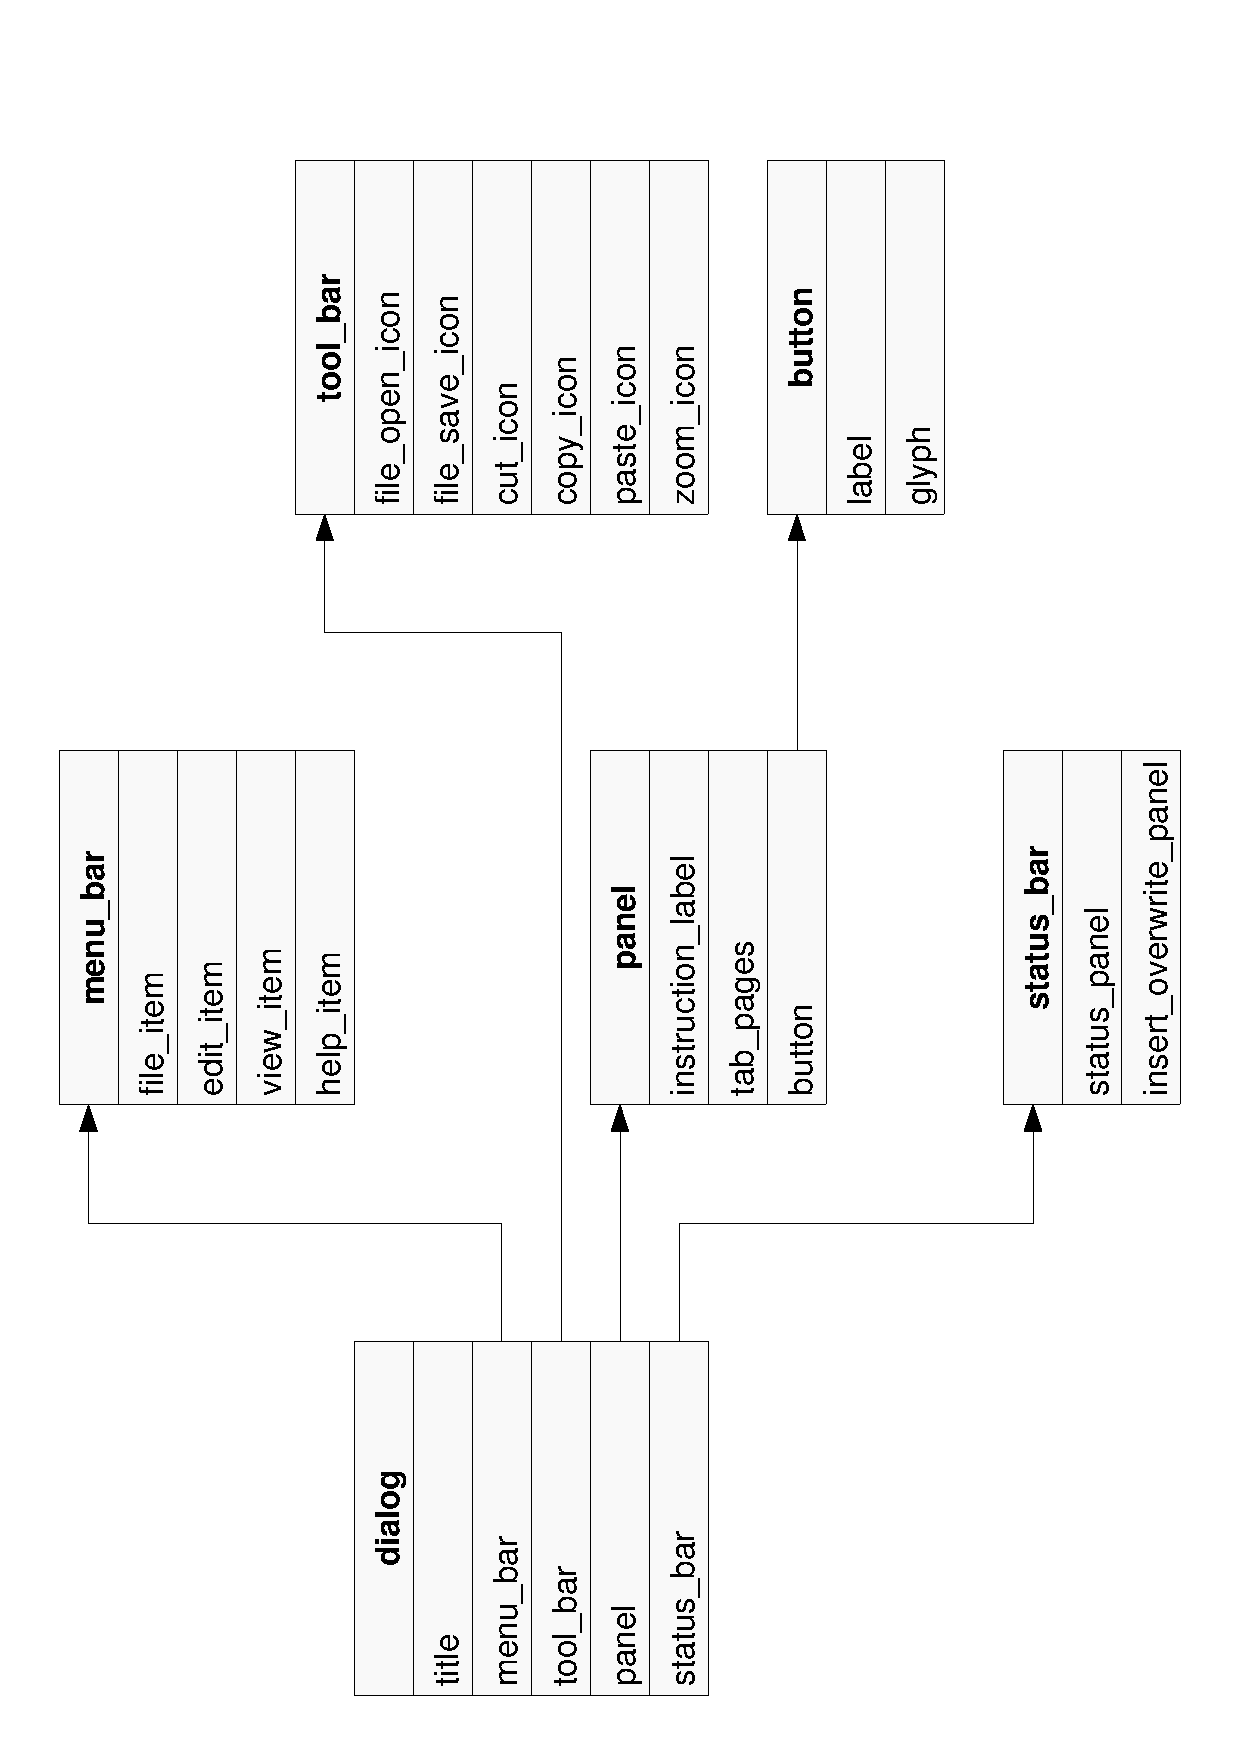
\includegraphics[scale=0.3,angle=-90]{graphic/td.pdf}
        \caption{CYBOL Template Diagram (TD) Proposal}
        \label{td_figure}
    \end{center}
\end{figure}

As said above, the four diagrams may look similar to their corresponding UML
pendant. For demonstration reasons, one possible proposal is given for each
diagram type. The TD (figure \ref{td_figure}) illustrates the same graphical
dialogue that was shown in the \emph{Template Editor} (figure
\ref{editor_figure}), in the previous section. The diagram looks pretty similar
to a UML CsD. Attributes and methods are not bundled in one concept though, and
inheritance does not exist. Associations are drawn if a concept links to an
external concept which may reside in another file (like the \emph{menu\_bar}),
for example. If a part (like the \emph{title}) is hold inline in the concept,
on the other hand, an association is not displayed. Upon clicking on a part in
a concept box, a dialogue opens up that allows the entry of meta data like the
part's channel, abstraction, model and further properties (details).

\begin{figure}[ht]
    \begin{center}
        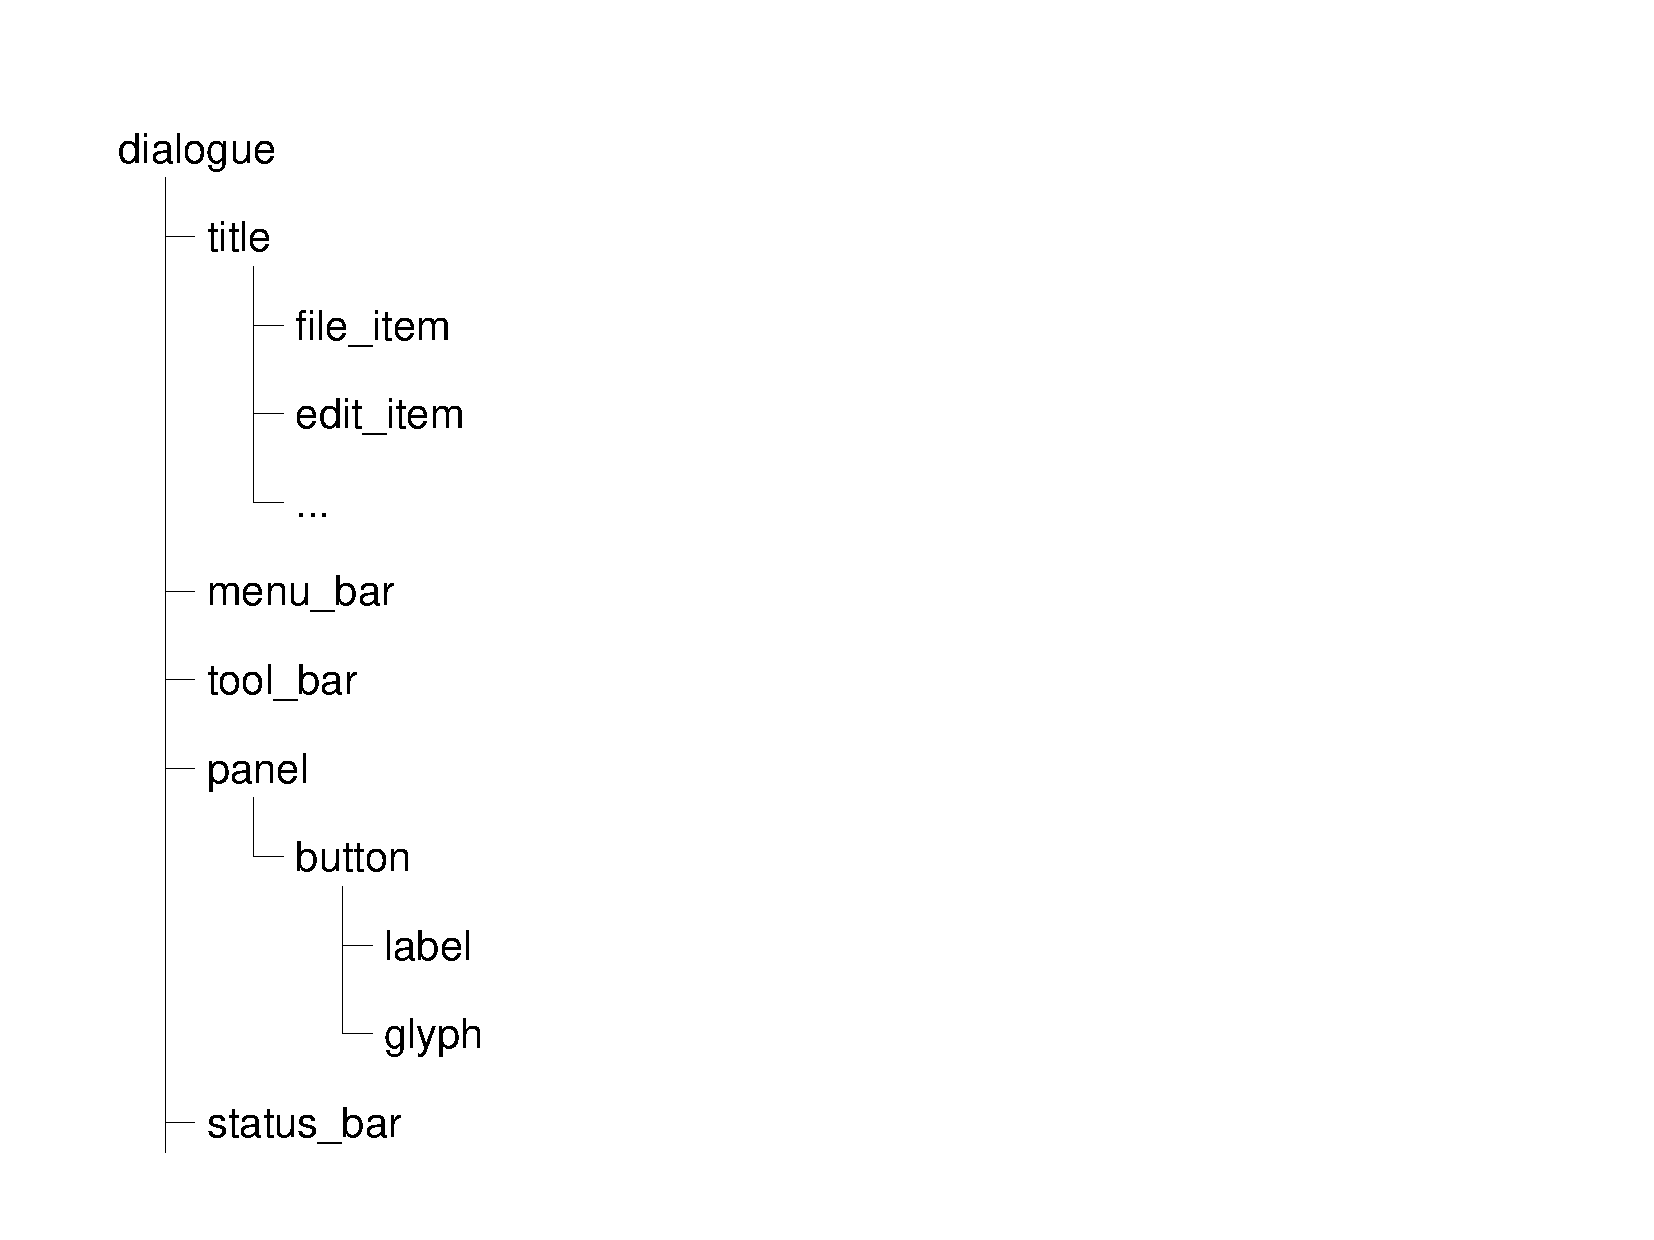
\includegraphics[scale=0.3,angle=-90]{graphic/md.pdf}
        \caption{CYBOL Model Diagram (MD) Proposal}
        \label{md_figure}
    \end{center}
\end{figure}

The MD (figure \ref{md_figure}) displays the runtime models that were
instantiated with knowledge templates providing the initial values. Again, the
parts of the graphical dialogue of figure \ref{editor_figure} are used in it.

\begin{figure}[ht]
    \begin{center}
        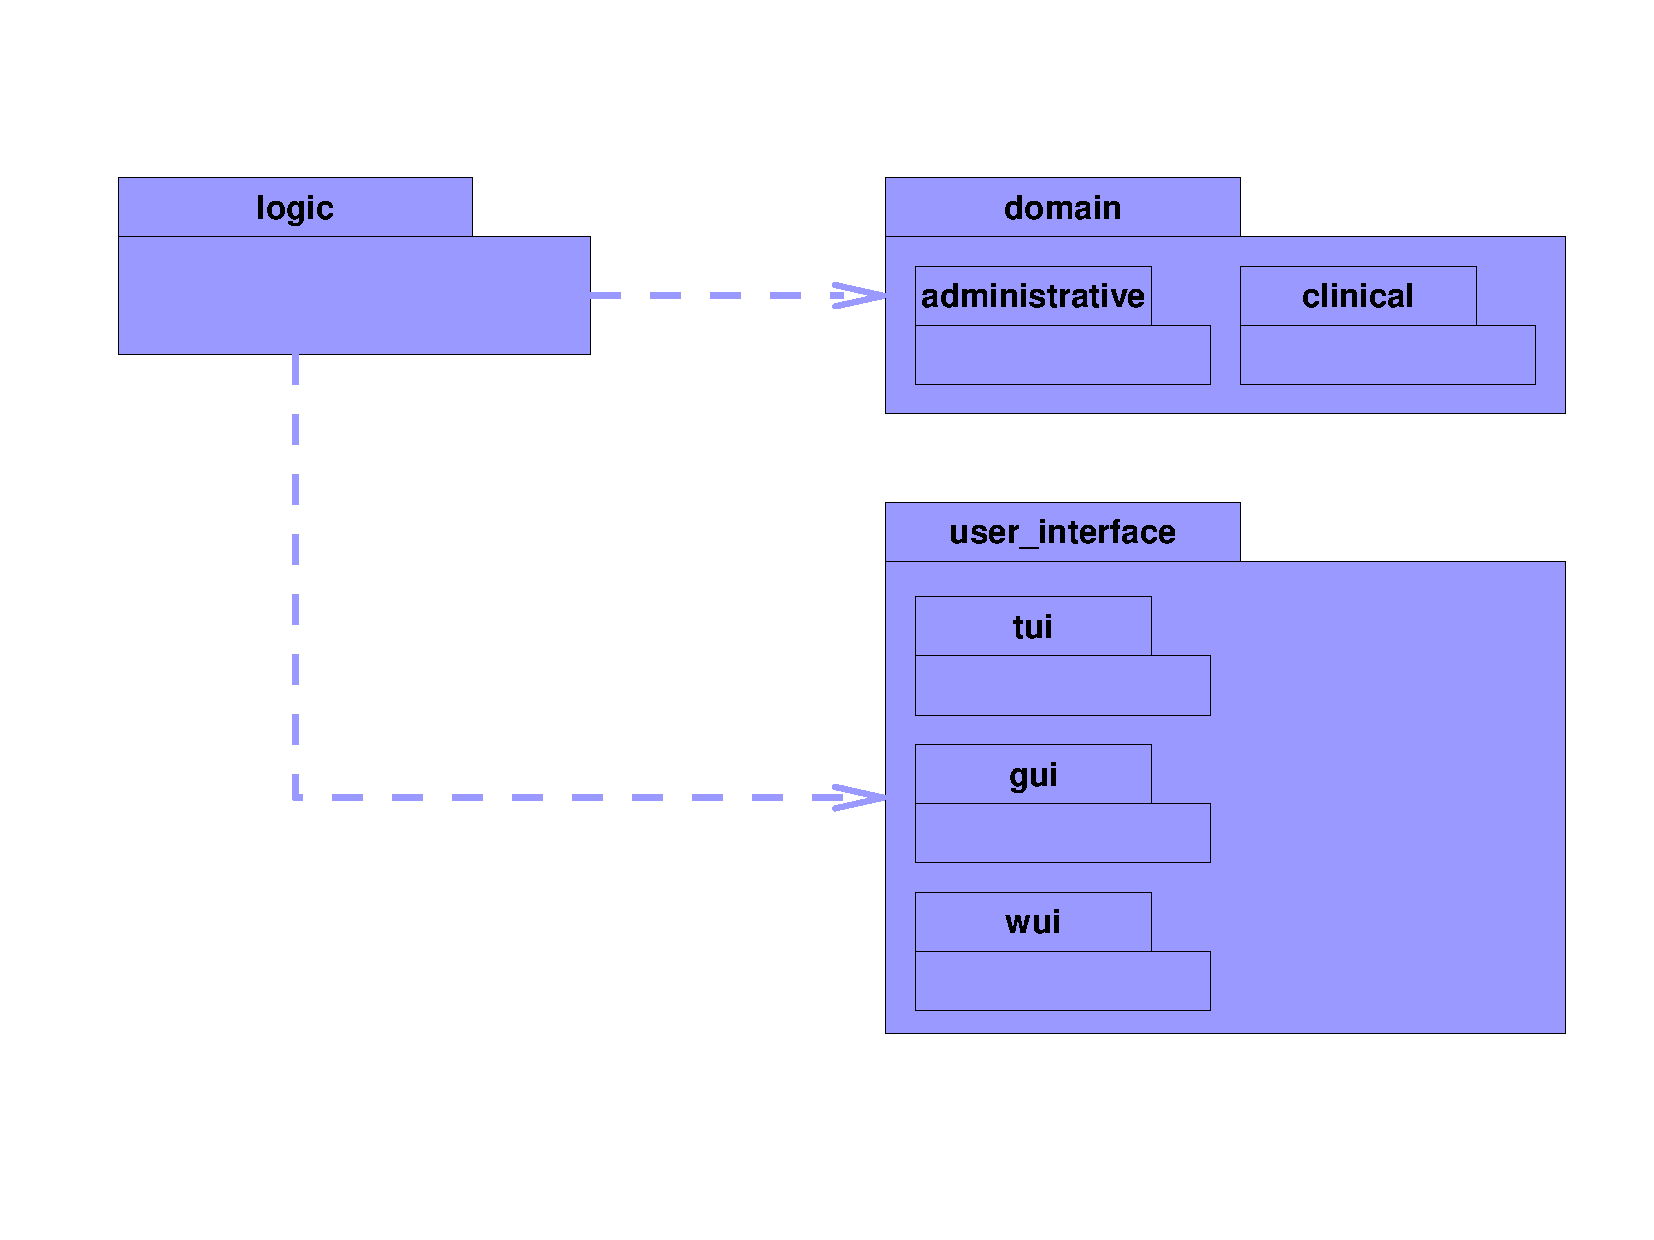
\includegraphics[scale=0.3,angle=-90]{graphic/od.pdf}
        \caption{CYBOL Organisation Diagram (OD) Proposal}
        \label{od_figure}
    \end{center}
\end{figure}

The OD (figure \ref{od_figure}) shows packages into which CYBOL knowledge
templates may be organised. Packages do normally correspond to directories on
file system level. The figure contains a \emph{domain} package consisting of
two sub packages, one containing knowledge templates for \emph{administrative}
patient data and the other holding templates for \emph{clinical} data of a
patient. Also, there is a \emph{User Interface} (UI) package containing three
sub packages, for: \emph{Textual UI} (TUI), \emph{Graphical UI} (GUI) and
\emph{Web UI} (WUI). Both, \emph{domain-} as well as \emph{user\_interface}
packages may be accessed from the operations residing in the \emph{logic}
package.

\begin{figure}[ht]
    \begin{center}
        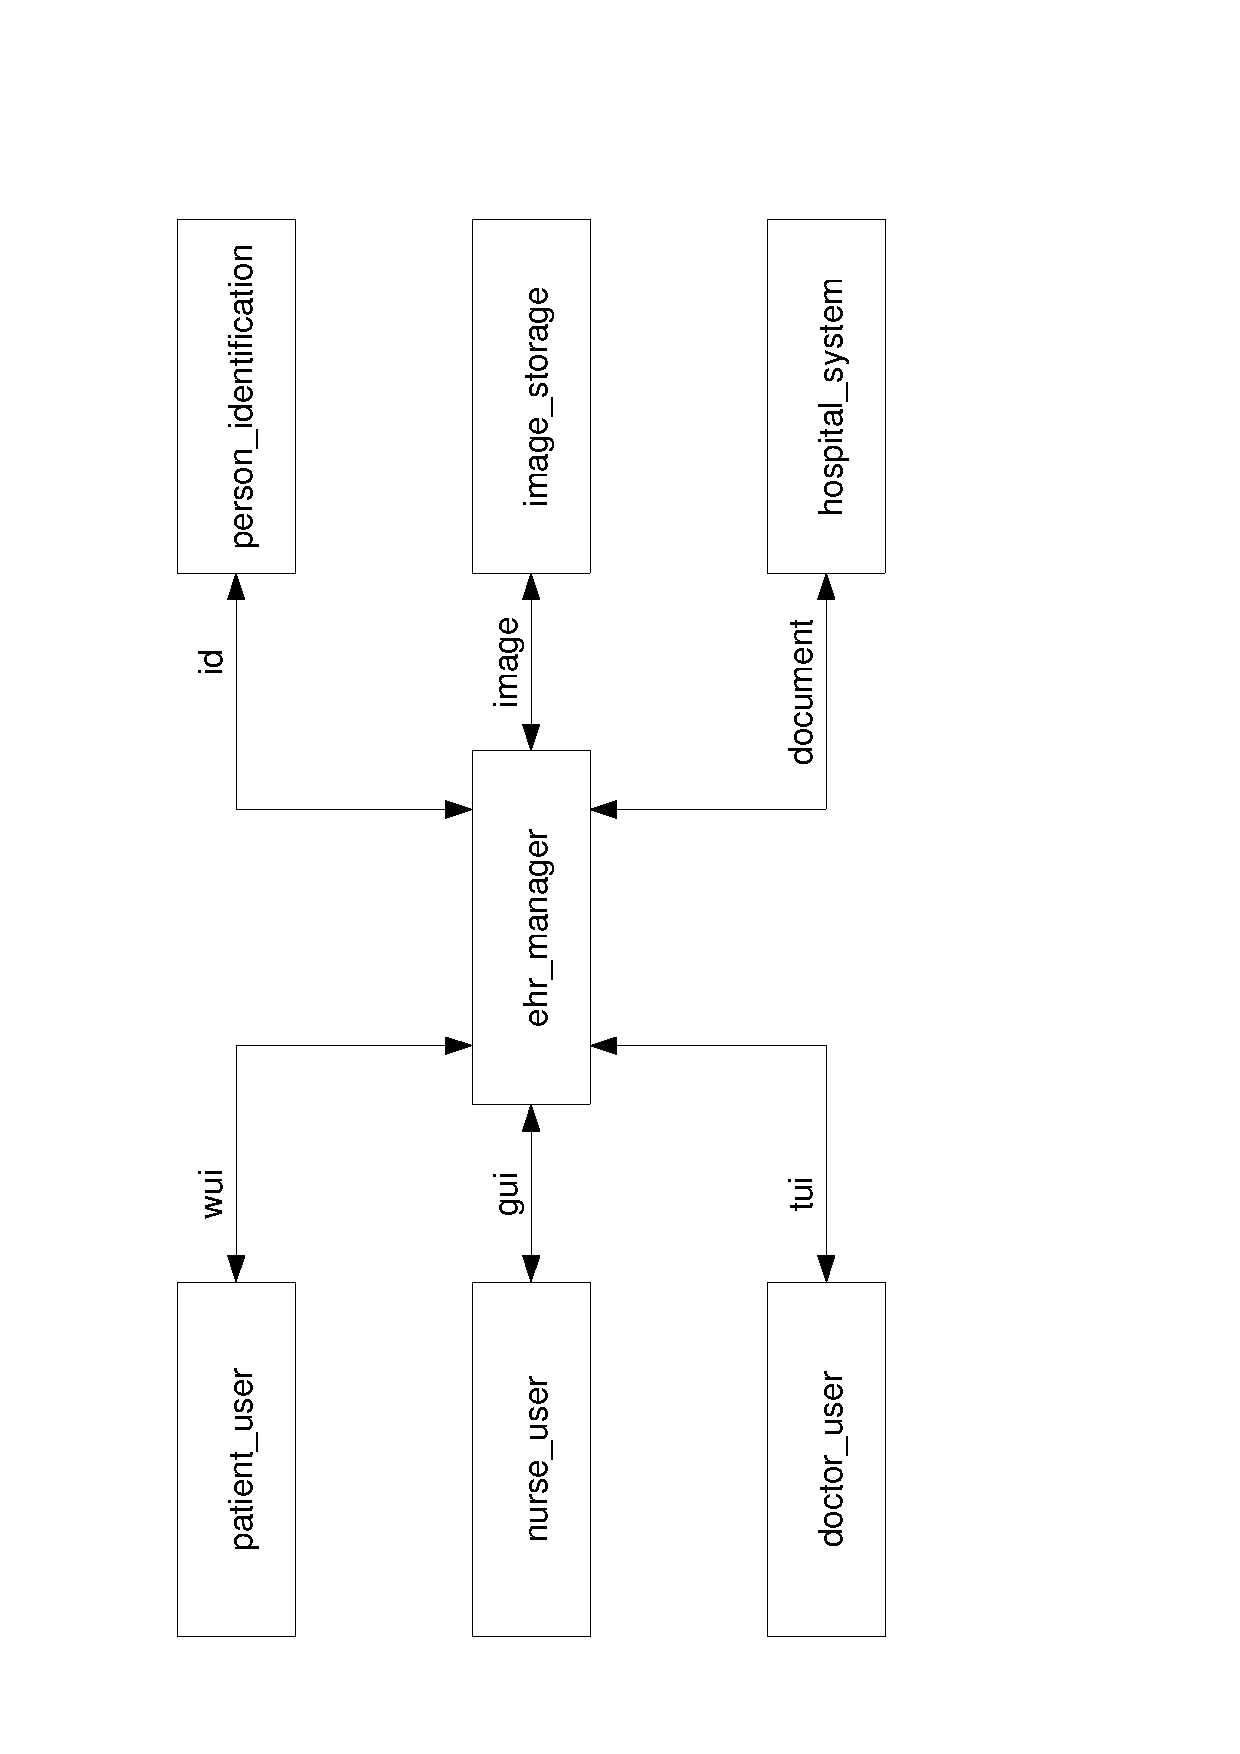
\includegraphics[scale=0.3,angle=-90]{graphic/cd.pdf}
        \caption{CYBOL Communication Diagram (CD) Proposal}
        \label{cd_figure}
    \end{center}
\end{figure}

The CD (figure \ref{cd_figure}), finally, shows a number of independent systems
communicating with each other. An \emph{Electronic Health Record} (EHR) manager
application may be found in the center of the figure. Patients communicate with
it using a WUI; nurses using a GUI and doctors using a TUI (for better
performance). A patient gets identified by asking a \emph{person\_identification}
service. Documents may be exchanged with a \emph{hospital\_system} and images
with a special \emph{image\_storage} system.

Besides these essential diagrams, additional ones may be used, of course. UML
diagrams like the AD, SD or TiD assist in modelling the flow of actions, that
is sequences of logic operations over time. Their ability to refine actions in
another level of granularity is of special interest. When removing the objects
bundled with method calls, they are well suitable for CYBOL. They use different
graphical elements, but in the end would store their knowledge in the same
templates. The transitions between different states of the runtime knowledge
tree over time are what the SMD wants to display. It may well be used with
CYBOL. But not only an application's behaviour over time is of interest, the
positions and expansions of its elements in space are as well important. This
mostly affects the design of user interfaces, graphical or textual. Designers
for these are therefore added to the list of useful diagrams. The usefulness of
feature model diagrams (section \ref{feature_model_heading}) for expressing
constraints that branches of the knowledge tree impose on each other could not
be investigated in this work, as this would break its frame.

Since CYBOL files contain all knowledge that is needed to define a complete
application system, the generation or parsing of classical source code is not
needed anymore, as chapter \ref{review_heading} will mention again. Therefore,
CYBOL knowledge design tools do only have to provide scanner- and generator
functionality for CYBOL (in order to formalise the knowledge designed as
semi-formal diagrams), but not for implementation languages.

%
% $RCSfile: model_viewer.tex,v $
%
% Copyright (C) 2002-2008. Christian Heller.
%
% Permission is granted to copy, distribute and/or modify this document
% under the terms of the GNU Free Documentation License, Version 1.1 or
% any later version published by the Free Software Foundation; with no
% Invariant Sections, with no Front-Cover Texts and with no Back-Cover
% Texts. A copy of the license is included in the section entitled
% "GNU Free Documentation License".
%
% http://www.cybop.net
% - Cybernetics Oriented Programming -
%
% http://www.resmedicinae.org
% - Information in Medicine -
%
% Version: $Revision: 1.1 $ $Date: 2008-08-19 20:41:07 $ $Author: christian $
% Authors: Christian Heller <christian.heller@tuxtax.de>
%

\subsection{Model Viewer}
\label{model_viewer_heading}
\index{CYBOL Model Viewer}
\index{CYBOL Runtime Model Editor}

Finally, it would be very helpful to have a tool displaying not just planned-,
but \emph{real} runtime statuses of the knowledge model tree, in other words a
\emph{live} memory snapshot displayed in a meaningful, hierarchical form. Such
a \emph{Model Viewer}, as it might be called, would not only help in debugging
applications, but could be extended towards a runtime \emph{Model Editor},
allowing to move whole knowledge tree branches from one parent node to another.


To what concerns the usage of existing UML tools for modelling CYBOL
applications, it has to be said that they are most likely not able to support
CYBOP models, nor can they be easily adapted. Even though the diagram
specifications may be similar, the underlying programming principles and model
repositories are just too different. It might be possible, however, to create
interfaces partly translating CYBOL-encoded (XML) models into UML models,
possibly using the \emph{XML Metadata Interchange} (XMI) standard or the like.
It will presumably be easier to translate CYBOL- into UML models, than vice
versa, because CYBOL is very expressive. While CYBOL knowledge templates
distinguish between whole-part- and meta elements, for example, UML models do
not. Another point is that CYBOL holds state- and logic knowledge in separate
templates, that would have to be merged into common classes when being
translated into UML. But the investigation and evaluation of further details
concerning the tool support is left for future works.

